%%%%%%%%%%%%%%%%%%%%%%%%%%%%%%%%%%%%%%%%%
% BA04 presentation 
% LaTeX Template
% Version 1.0 (14/12/14)
%
% This template has been downloaded from:
% http://www.LaTeXTemplates.com
%
% License:
% CC BY-NC-SA 3.0 (http://creativecommons.org/licenses/by-nc-sa/3.0/)
%
%%%%%%%%%%%%%%%%%%%%%%%%%%%%%%%%%%%%%%%%%

%----------------------------------------------------------------------------------------
%	PACKAGES AND THEMES
%----------------------------------------------------------------------------------------

\documentclass{beamer}

\mode<presentation> {

% The Beamer class comes with a number of default slide themes
% which change the colors and layouts of slides. Below this is a list
% of all the themes, uncomment each in turn to see what they look like.

%\usetheme{default}
%\usetheme{AnnArbor}
%\usetheme{Antibes}
%\usetheme{Bergen}
%\usetheme{Berkeley}
%\usetheme{Berlin}
%\usetheme{Boadilla}
%\usetheme{CambridgeUS}
%\usetheme{Copenhagen}
%\usetheme{Darmstadt}
%\usetheme{Dresden}
%\usetheme{Frankfurt}
%\usetheme{Goettingen}
%\usetheme{Hannover}
%\usetheme{Ilmenau}
%\usetheme{JuanLesPins}
%\usetheme{Luebeck}
\usetheme{Madrid}
%\usetheme{Malmoe}
%\usetheme{Marburg}
%\usetheme{Montpellier}
%\usetheme{PaloAlto}
%\usetheme{Pittsburgh}
%\usetheme{Rochester}
%\usetheme{Singapore}
%\usetheme{Szeged}
%\usetheme{Warsaw}

% As well as themes, the Beamer class has a number of color themes
% for any slide theme. Uncomment each of these in turn to see how it
% changes the colors of your current slide theme.
\usepackage{color}
%\usecolortheme{albatross}
%\usecolortheme{beaver}
%\usecolortheme{beetle}
%\usecolortheme{crane}
%\usecolortheme{dolphin}
%\usecolortheme{dove}
%\usecolortheme{fly}
%\usecolortheme{lily}
%\usecolortheme{orchid}
\usecolortheme{rose}
%\usecolortheme{seagull}
%\usecolortheme{seahorse}
%\usecolortheme{whale}
%\usecolortheme{wolverine}
\usepackage{tikz}
\usetikzlibrary{calc}
\usepackage{multirow}
\usepackage{adjustbox}
\usepackage{tabularx}
\newcolumntype{b}{X}
\newcolumntype{s}{>{\hsize=.5\hsize}X}

% tikzmark command, for shading over items
\newcommand{\tikzmark}[1]{\tikz[overlay,remember picture] \node (#1) {};}
%\setbeamertemplate{footline} % To remove the footer line in all slides uncomment this line
\setbeamertemplate{footline}[page number] % To replace the footer line in all slides with a simple slide count uncomment this line

\setbeamertemplate{navigation symbols}{} % To remove the navigation symbols from the bottom of all slides uncomment this line
}


\AtBeginSection[]{
  \begin{frame}
  \vfill
  \centering
  \begin{beamercolorbox}[sep=8pt,center,shadow=true,rounded=true]{title}
    \usebeamerfont{title}\insertsectionhead\par%
  \end{beamercolorbox}
  \vfill
  \end{frame}
}
\usepackage{graphicx} % Allows including images
\usepackage{booktabs} % Allows the use of \toprule, \midrule and \bottomrule in tables
\usepackage[english]{babel}
\usepackage[utf8x]{inputenc}
\bibliographystyle{alpha}

\usepackage{algorithm}
\usepackage{algorithmicx}
\usepackage[noend]{algpseudocode}
\algnewcommand\algorithmicdef{\textbf{}}
\algnewcommand\DEF{\item[\algorithmicdef]}

\algnewcommand\algorithmic{\textbf{Input:}}
\algnewcommand\INPUT{\item[\algorithmicinput]}

\algnewcommand\algorithmicinputitem{}
\algnewcommand\INPUTITEM{\item[\algorithmicinputitem]}

\newcommand{\ntronitemsep}{1em}


%TIKZ MAGIC, Stolen from http://tex.stackexchange.com/questions/15735/adding-arrows-to-each-term-of-an-equation

\usepackage{amsmath}
\usepackage{tikz}
\usetikzlibrary{arrows}

% Define how TiKZ will draw the nodes
\tikzset{mathterm/.style={draw=black,fill=white,rectangle,anchor=base}}
\tikzstyle{every picture}+=[remember picture]
\everymath{\displaystyle}

\makeatletter

% Designate a term in a math environment to point to
% Syntax: \mathterm[node label]{some math}
\newcommand\mathterm[2][]{%
   \tikz [baseline] { \node [mathterm] (#1) {$#2$}; }}

% A command to draw an arrow from the current position to a labelled math term
% Default color=black, default arrow head=stealth
% Syntax: \indicate[color]{term to point to}[path options]
\newcommand\indicate[2][black]{%
   \tikz [baseline] \node [inner sep=0pt,anchor=base] (i#2) {\vphantom|};
   \@ifnextchar[{\@indicateopts{#1}{#2}}{\@indicatenoopts{#1}{#2}}}
\def\@indicatenoopts#1#2{%
   {\color{#1} \tikz[overlay] \path[line width=1pt,draw=#1,-stealth] (i#2) edge (#2);}}
\def\@indicateopts#1#2[#3]{%
   {\color{#1} \tikz[overlay] \path[line width=1pt,draw=#1,-stealth] (i#2) [#3] edge (#2);}}


\DeclareMathOperator*{\argmax}{arg\!max}

\makeatother


%----------------------------------------------------------------------------------------
%	TITLE PAGE
%----------------------------------------------------------------------------------------

\title[Numerical Relation Extraction with Minimal Supervision]{Numerical Relation Extraction with Minimal Supervision} % The short title appears at the bottom of every slide, the full title is only on the title page
\subtitle{MTP Presentation}
\author[]{Aman Madaan \and Ashish Mittal}
\institute[]{
  Indian Institute of Technology Bombay, Mumbai
}
\date{25th June, 2015}
\begin{document}

\begin{frame}
\titlepage % Print the title page as the first slide
\end{frame}

\begin{frame}
\frametitle{Outline} % Table of contents slide, comment this block out to remove it
\tableofcontents % Throughout your presentation, if you choose to use \section{} and \subsection{} commands, these will automatically be printed on this slide as an overview of your presentation
\end{frame}

%----------------------------------------------------------------------------------------
%	PRESENTATION SLIDES
%----------------------------------------------------------------------------------------

%------------------------------------------------
\section{Introduction} % Sections can be created in order to organize your presentation into discrete blocks, all sections and subsections are automatically printed in the table of contents as an overview of the talk
%PART 1 : Motivation
\begin{frame}{Entities have Numerical Attributes}

    \begin{figure}
    \centering
    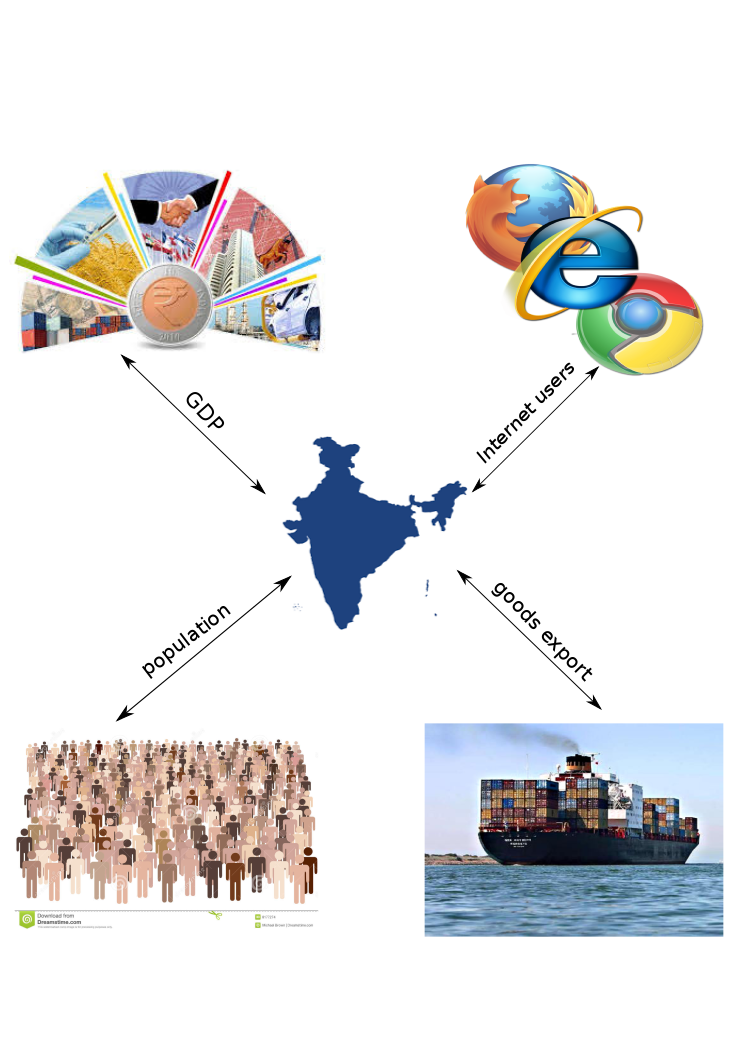
\includegraphics[width = 0.5\textwidth]{images/motivation}
  \end{figure}
 
\end{frame}

\begin{frame}{Entities have Numerical Attributes}
 \begin{center}
 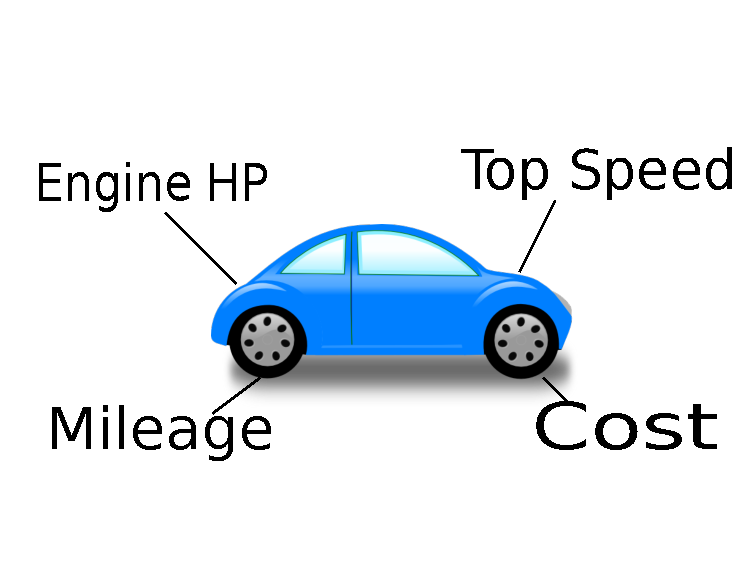
\includegraphics[scale=0.45]{images/car.pdf}
 % car.pdf: 363x272 pixel, 72dpi, 12.81x9.60 cm, bb=0 0 363 272
\end{center}

\end{frame}

\begin{frame}{Entities and Numerical Attributes}
 
 \begin{itemize}

  \item For popular entities, finding complete knowledge bases is possible. \pause \\~\\
  \item data.worldbank.org, Wikipedia infoboxes, freebase ... \pause \\~\\
  \item What about less popular entities?  \pause 
    \begin{itemize}
      \item What is the population of Arbit Apartments, Powai? \pause \\~\\
      \item What is the GDP of Sugarcane Industry of India? \pause \\~\\
      \item Percent of Internet users in Mumbai? 
    \end{itemize}
 \end{itemize} 
\end{frame}

\begin{frame}{Motivation}
 \begin{figure}[h]
 \centering
 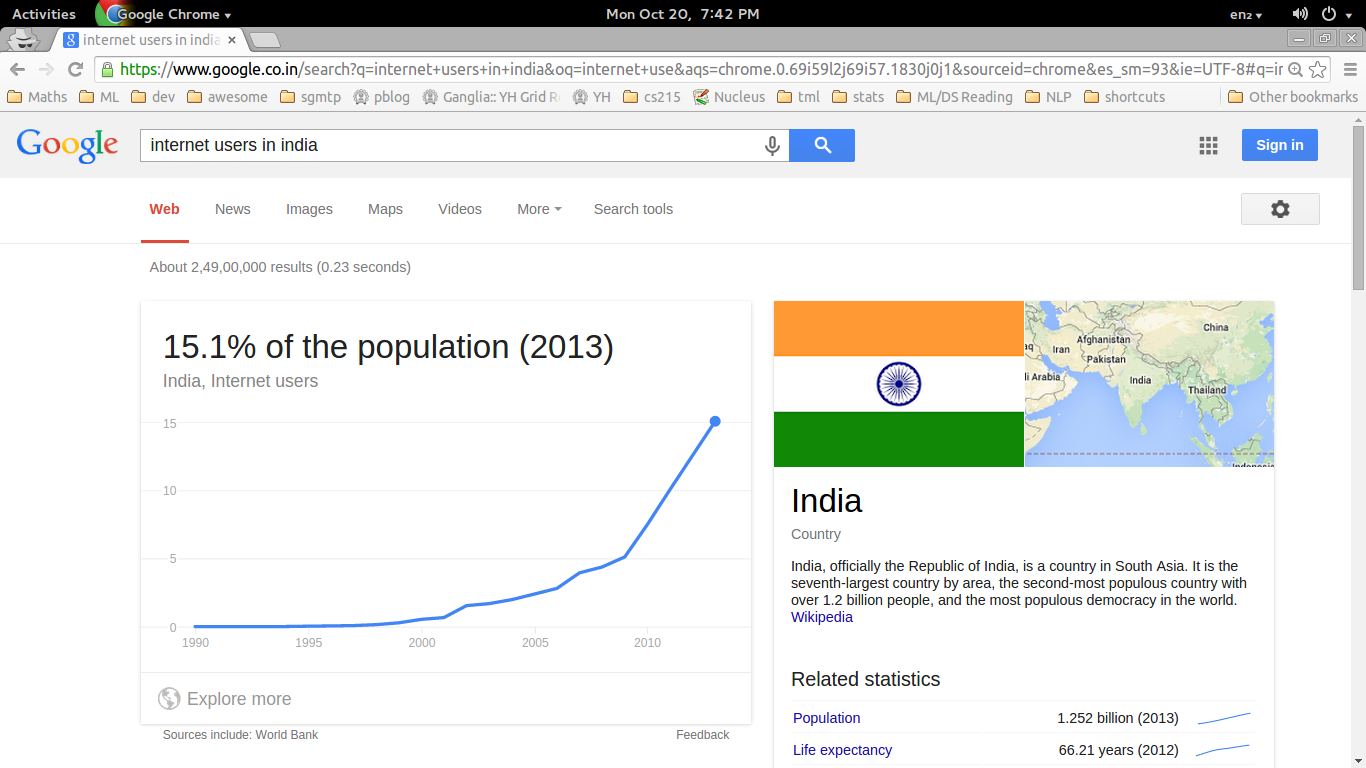
\includegraphics[bb=0 0 1366 741,scale=0.25]{images/resultindia.png}
 % resultindia.png: 1366x741 pixel, 72dpi, 48.19x26.14 cm, bb=0 0 1366 741
\end{figure}
\end{frame}

\begin{frame}{Motivation}
 \begin{figure}[h]
 \centering
 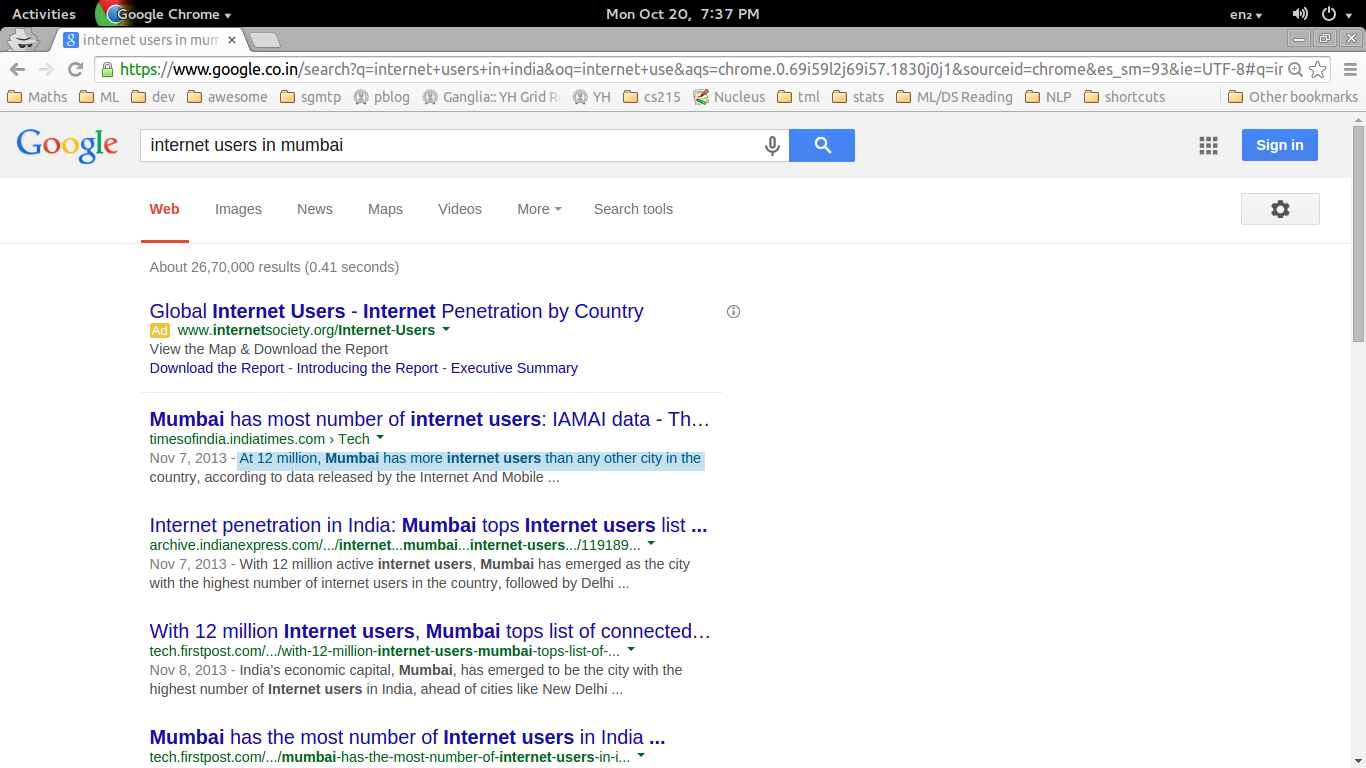
\includegraphics[bb=0 0 1366 741,scale=0.25]{images/resultmumbai.png}
 % resultindia.png: 1366x741 pixel, 72dpi, 48.19x26.14 cm, bb=0 0 1366 741
\end{figure}
\end{frame}

\begin{frame}{Motivation}

\begin{itemize}
 \item  Web is huge.  \pause \\~\\
 \item Probably, there is some page which contains the information we are looking for. \pause \\~\\
 \item The way in which you express a fact about an entity depends on the fact, and not the entity. \pause \\~\\
 \item We may expect \textbf{the sentence structure} \footnote{More on this in the coming slides} to be similar. \pause
 \begin{itemize}
    \item Population of India reached 1.3 billion, making it the second largest country in the world. \pause \\~\\
    \item Population of Arbit Apartments, Powai reached 1300.
 \end{itemize}
 
\end{itemize}
\end{frame}



% \section*{Problem Statement}
% \begin{frame}{Problem Statement}
%  \begin{itemize}
%   \item Given that we know a lot of facts about some entities, can we train extractors that run over the web and pull similar facts about other entities?
%  \end{itemize}
% \end{frame}

\begin{frame}{Problem Statement}

\begin{itemize}
 
 \item  The knowledge is scattered in unstructured text on the Web.
 \begin{figure}[h]
 \centering
 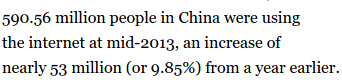
\includegraphics[bb=0 0 1139 53,scale=0.47]{images/ex_2.png}
 % ex_1.png: 1139x53 pixel, 72dpi, 40.18x1.87 cm, bb=0 0 1139 53
\end{figure}

 \begin{figure}[h]
 \centering
 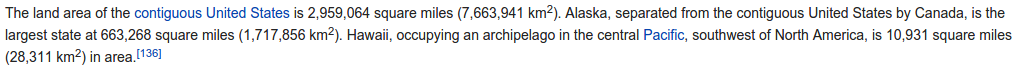
\includegraphics[bb=0 0 1139 53,scale=0.30]{images/ex_3.png}
 % ex_1.png: 1139x53 pixel, 72dpi, 40.18x1.87 cm, bb=0 0 1139 53
\end{figure}


  \item Can such facts be extracted automatically?
\end{itemize}

\end{frame}
\begin{frame}{Problem Statement}
\begin{itemize}
 \item Formally, train extractors that can harness the Web for numerical relations, where relations are 3-tuples linking an entity
to a number \\~\\
   
    \begin{itemize}
	\item  (India, \textbf{economy}, 1.842 trillion USD) \\~\\
	\item  (China, \textbf{internet users},  590.56 million) \\~\\
	\item  (USA, \textbf{land area}, 2,959,054 square mile)
    \end{itemize}

 \end{itemize}
\end{frame}

%PART 2 : Relation extraction as a machine learning problem

\section{Relation Extraction as a Machine Learning Problem}

\begin{frame}{Relation Extraction as a Machine Learning Problem}
 \begin{itemize}
  \item \textbf{Structure} and \textbf{content} of sentences expressing the same relations can be \emph{expected} to be similar.  \\~\\
 \begin{itemize}
      \item The population of Australia is estimated to be 23,622,400 as of 7 October 2014. \\~\\
      \item According to an official estimate for 1 June 2014, the population of Russia is 143,800,000.   
   \end{itemize}   
 \end{itemize}
\end{frame}
\begin{frame}{Relation Extraction as a Machine Learning Problem}
\begin{itemize}
\item \textbf{Structure} and \textbf{content} of sentences expressing the same relations can be \emph{expected} to be similar.  \\~\\
 \begin{itemize}   
    \item At 17,075,400 square kilometres, Russia is the largest country in the world. \\~\\
    \item With an area of 504,030 $km^{2}$, Spain is the second largest country in Western Europe. 
    \end{itemize}
 \end{itemize}
\end{frame}
\begin{frame}{Relation Extraction as a Machine Learning Problem}
 
 \begin{itemize}
  \item Redundancy in grammatical features and dependencies of the sentences expressing same relation. \pause 
     \begin{figure}
    \centering
    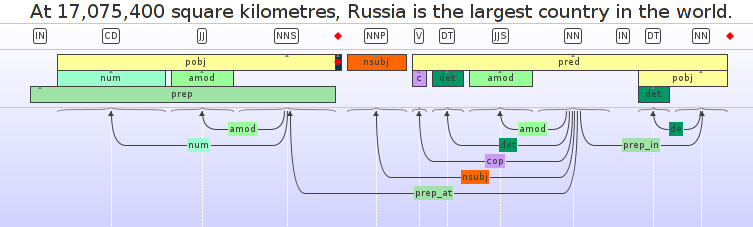
\includegraphics[width = 0.8\textwidth]{images/ex_4}
  \end{figure} \pause
  
   \begin{figure}
    \centering
    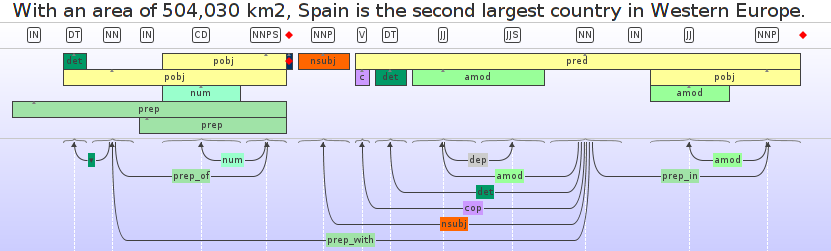
\includegraphics[width = 0.8\textwidth]{images/ex_5}
  \end{figure}
 \end{itemize}

\end{frame}


\begin{frame}{Possible Workflow} \pause

\begin{algorithmic}[1]
\State \textbf{Collect enough examples} for each relation so that there are sufficient patterns and enough redundancy to exploit.
\item[]
\State \textbf{Extract features} (important keywords, grammatical structure, parse trees, etc.) for these sentences.
\item[]
\State \textbf{Train} a multi-class classifier on this training data.
\item[]
\For{$sentence\ s \in Corpus $}
\State \textbf{Extract} features for $s$.
\State \textbf{Predict} the relation using the model for these features.
\State \textbf{Store} the fact into a database.
\EndFor
\end{algorithmic}
\end{frame}

\begin{frame}{Challenge}
 \begin{itemize}
  \item Large Corpus ($\sim$16 million sentences), hand labeling is out of question \pause \\~\\
  \item Need lots of training data to learn high quality extractors \pause \\~\\
  \item What makes this problem interesting?
 \end{itemize}
\end{frame}

%---------------------------------

%\begin{frame}{Related Work}
% \begin{itemize}
% \setlength \itemsep{2em}
%  \item Mintz et. el [2009], were the first ones to use distant supervision for relation extraction from the text.
%  \item Traditional IE deals with relations having both the arguments that are entities (e.g, Microsoft, Bill Gates).
%  \item Riedel et. al[2010] were the first ones to use graphical model for relation extraction.
%  \item Later systems MultiR (Hoffman et. al[2011]) improved upon the graphical model by improving upon the distant supervision assumption.
  
% \end{itemize}
%\end{frame}

%------------------------



% A subsection can be created just before a set of slides with a common theme to further break down your presentation into chunks

\section{Peculiarities of Numerical Relation Extraction}
\begin{frame}
\frametitle{Peculiarities of Numerical Relation Extraction}
\framesubtitle{Numbers are weak entities}
\begin{itemize}
\item Quantities can appear in far more contexts than typical entities. ("Bill Gates", "Microsoft") vs. ("11", "Microsoft")
\item Regular IE have fewer cases of entity disambiguation as compared to numerical IE
\end{itemize}

\begin{figure}
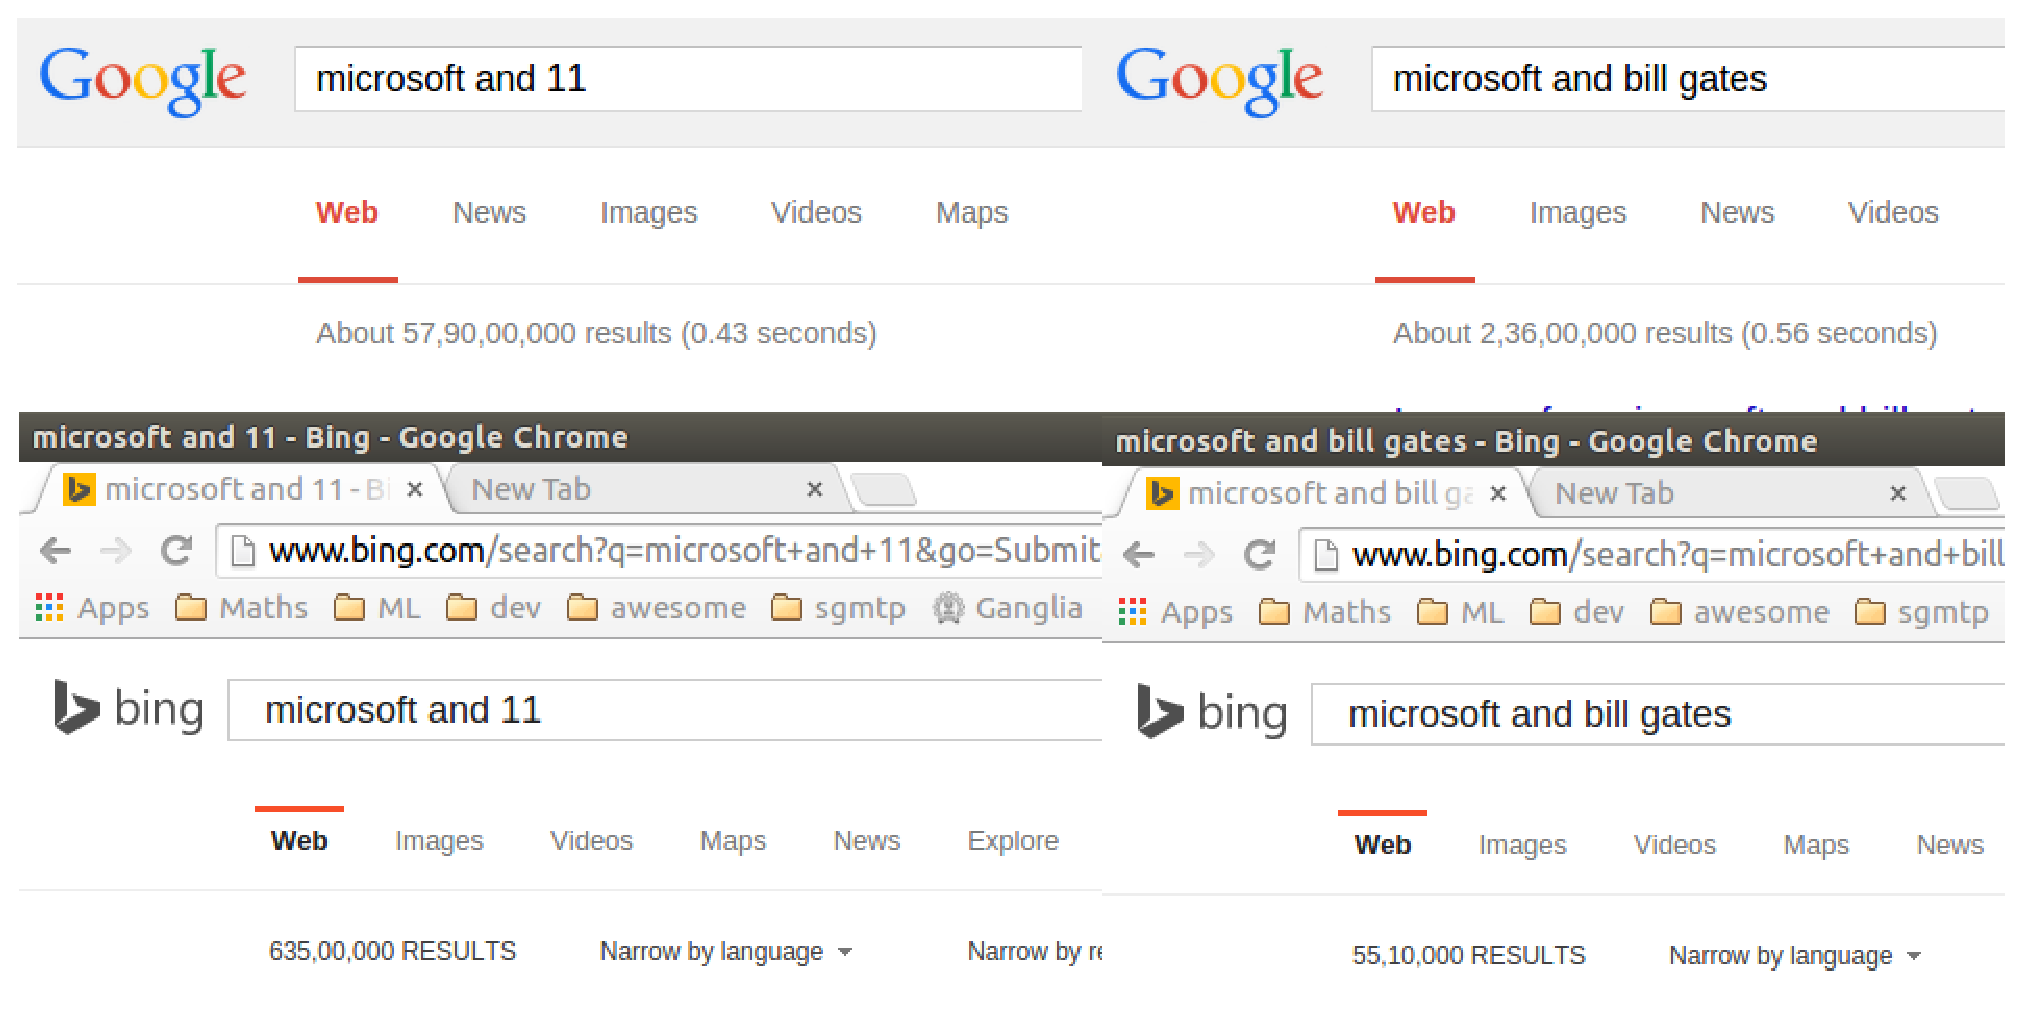
\includegraphics[width=0.7\textwidth]{images/popularitynumbers.eps}
\end{figure}

\end{frame}
    
\begin{frame}
\frametitle{Peculiarities of Numerical Relation Extraction}
\framesubtitle{Numbers are weak entities}
\begin{itemize}
 \item Noise is more for the small whole numbers that are unit\-less or with popular units (e.g, percent)
 \item 1 or 5\% vs. 11.42145 or 330 m/sec
\end{itemize}

\begin{center}
\begin{tabular}{l|l}
Number & Frequency (Avg. 57.84)\\ \hline
3 & 85333\\
20 & 86359\\
2 & 91608\\
1 & 100014\\
10 & 100780
\end{tabular}
\end{center}
\end{frame}


\begin{frame}
\frametitle{Peculiarities of Numerical Relation Extraction}
\framesubtitle{Units}
\begin{itemize}
\setlength \itemsep{1em}
\item Unit acts as types for numbers.
\item Same quantity may be expressed with different unit
	\begin{itemize}
    	\item 20 kms or 12.4 miles
   	\end{itemize}
\item Unit extractor needs to perform unit conversions for correct matching and extraction
\end{itemize}
\end{frame}

\begin{frame}
\frametitle{Peculiarities of Numerical Relation Extraction}
\framesubtitle{Delta Words}

\begin{itemize}
\setlength \itemsep{1em}
\item Not uncommon to find sentences expressing change in the value of a relation (instead of, or in addition to, the actual value).
\begin{itemize}
\setlength \itemsep{1em}
\item Amazon stock price \textit{\color{red}increased by} \$35 to close at \$510.
\item India's tiger population sees 30\% \textit{\color{red}increase}.
\item Ford poised to raise dividend by 20\% even as profit declines.
\end{itemize}
\end{itemize}
\end{frame}

\begin{frame}
\frametitle{Peculiarities of Numerical Relation Extraction}
\framesubtitle{Relation/Argument Scoping}

\begin{itemize}
\setlength \itemsep{1em}
\item Additional modifiers to arguments or relation words may subtly change the meaning and confuse the extractor.
\begin{itemize}
\setlength \itemsep{1em}
\item \emph{rural} literacy rate of India
\item literacy rate of \emph{rural} India
\end{itemize}
\item The modifiers are usually adjectival modifiers
\end{itemize}

\end{frame}

\begin{frame}
\frametitle{Peculiarities of Numerical Relation Extraction}
\framesubtitle{Keywords}

\begin{itemize}
\setlength \itemsep{1em}
\item Sentences expressing many numerical relations usually include one or a handful of keywords.
\item Sentences expressing the GDP of a country with mentioning the term \textit{GDP}? Sentences expressing inflation without mentioning inflation?
\item \textit{Founder of} without the phrase \textit{founder of}?
\begin{itemize}
\item Bill Gates is the founder of Microsoft
\item Bill Gates founded Microsoft
\item Bill Gates is the father of Microsoft
\item Bill Gates laid the foundation stone of Microsoft
\item Bill Gates started Microsoft
\end{itemize}
\end{itemize}

\end{frame}


\section{NumberRule: Rule Based Relation Extraction}
%------------------------------------------------

\begin{frame}
\frametitle{Rule Based IE}
\framesubtitle{Academia vs. Industry}

\begin{figure}
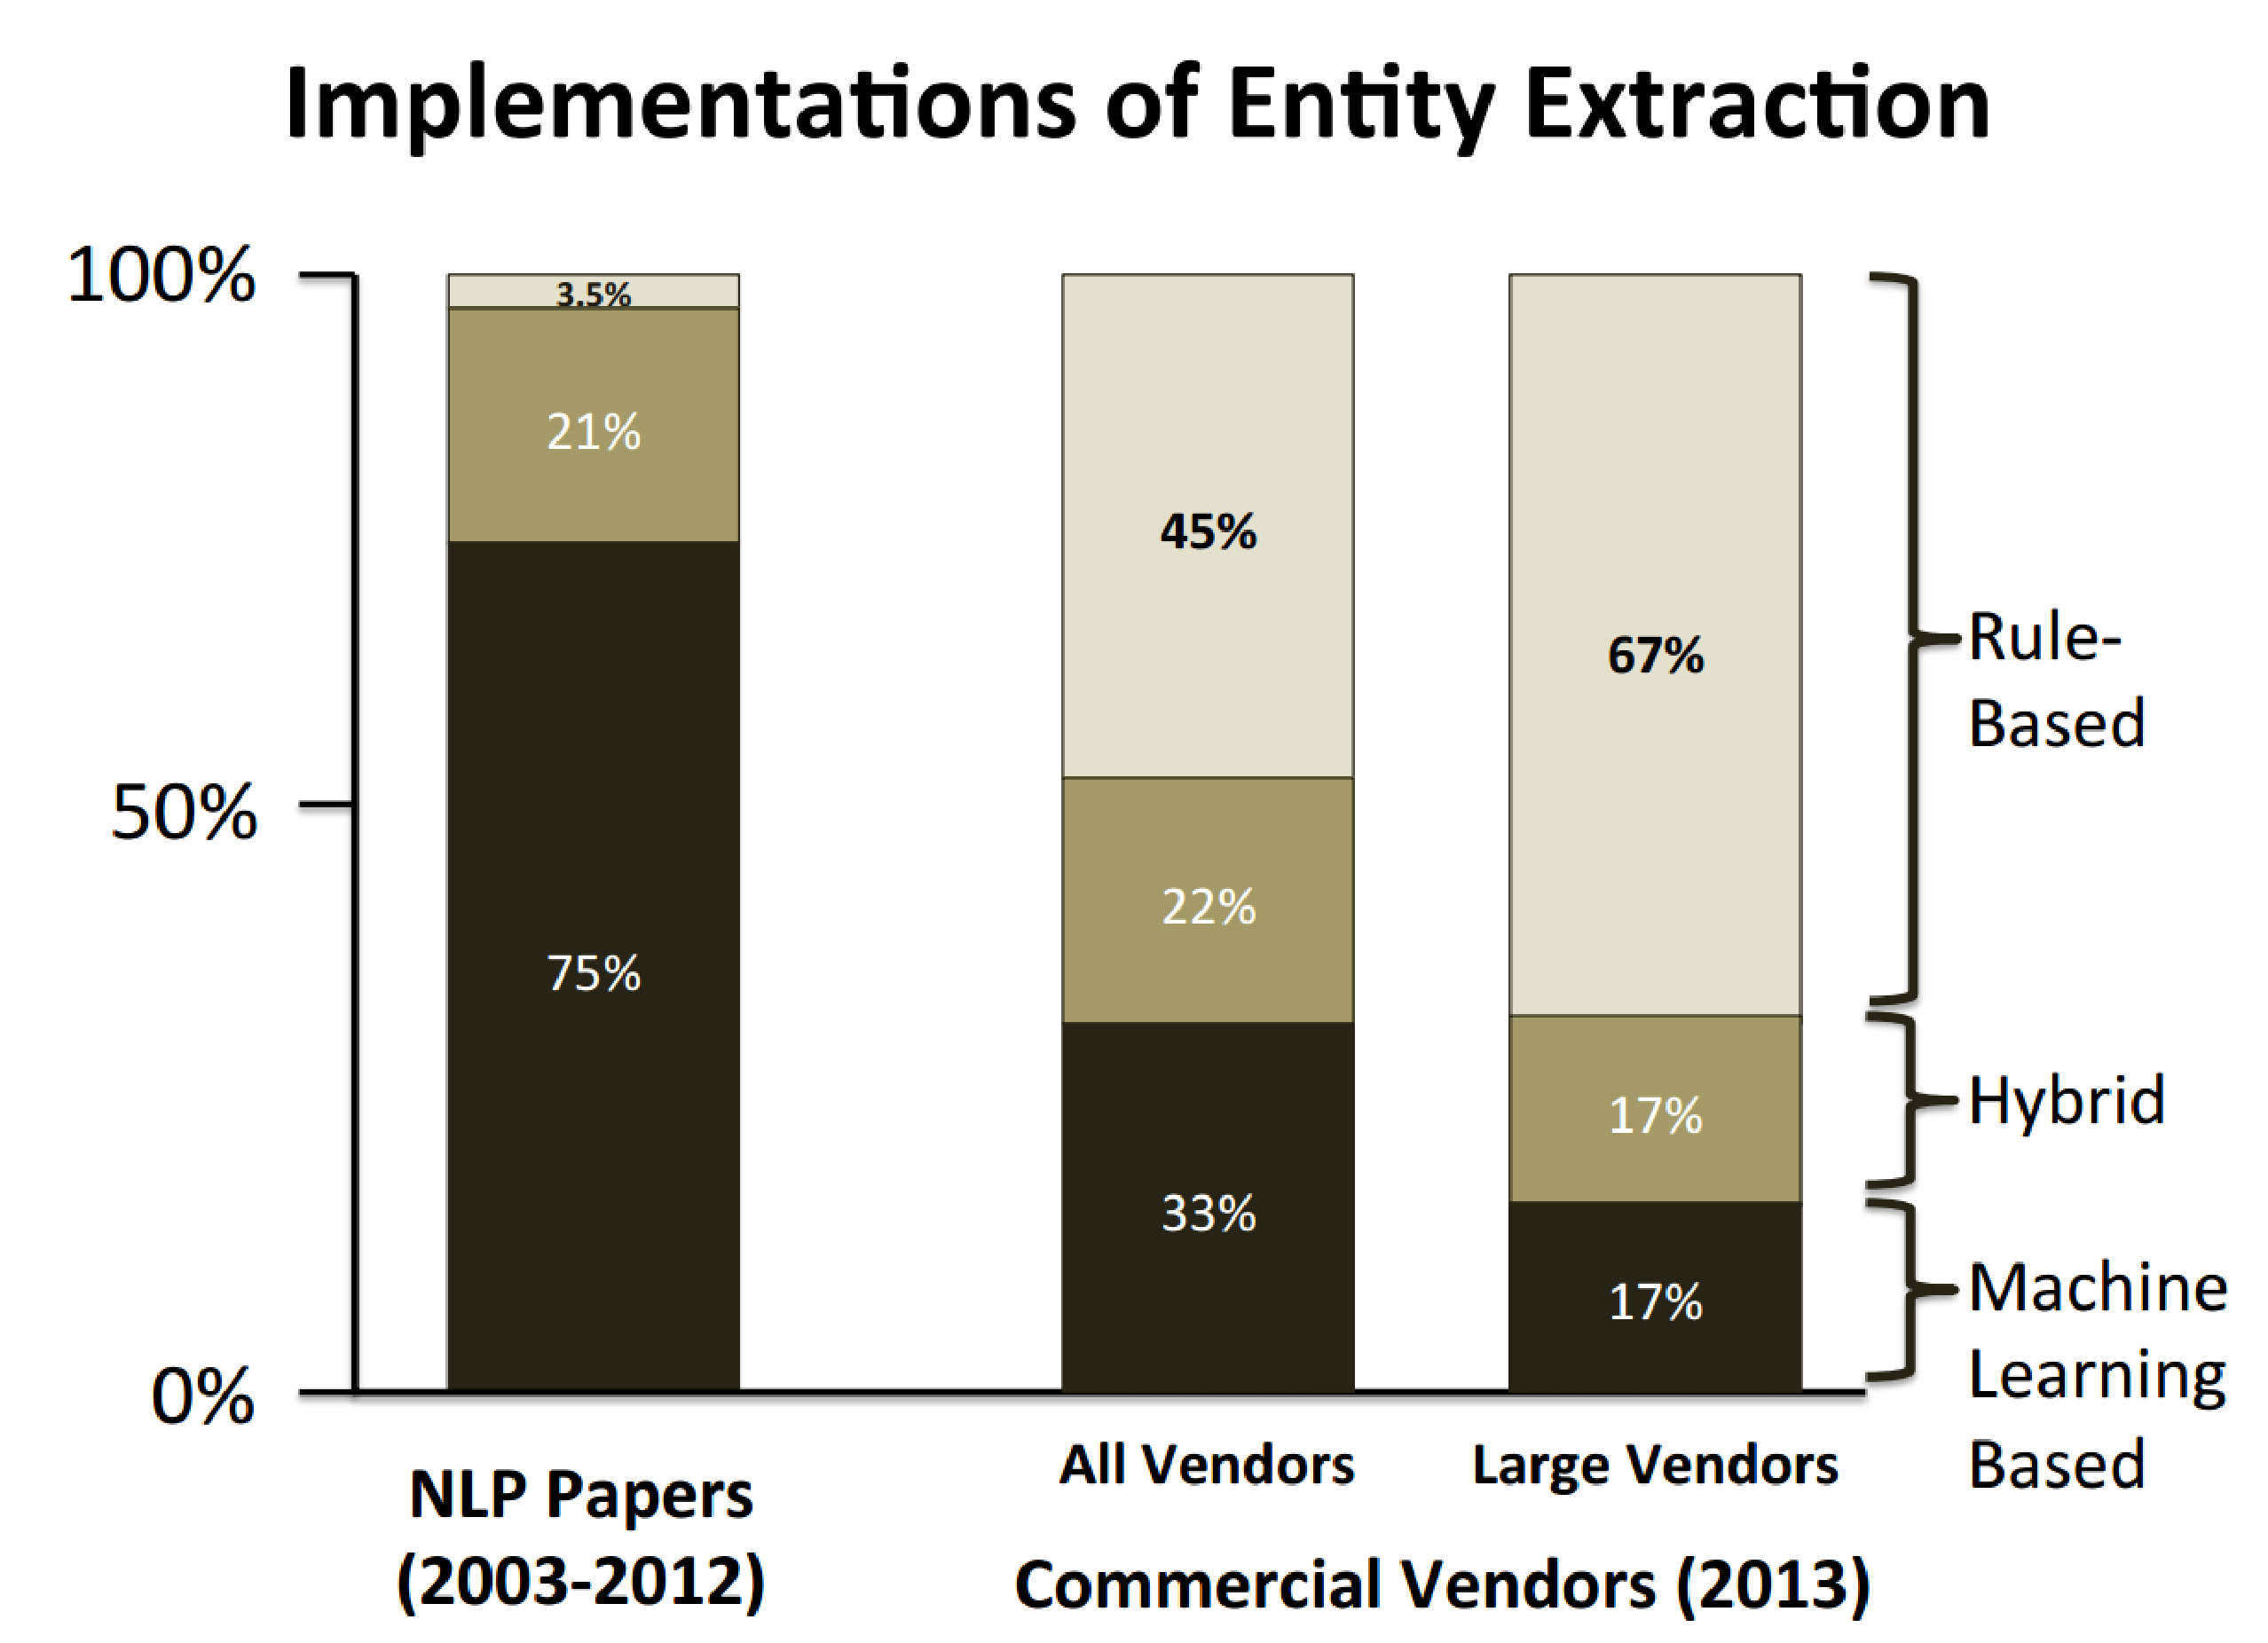
\includegraphics[width=0.7\textwidth]{images/longliverulebased.eps}
\end{figure}

\footnote{from \cite{chiticariu2013rule}}

\end{frame}
%------------------------------------------------

\begin{frame}
 \frametitle{NumberRule}
 \framesubtitle{Dependencies in NLP}
 \begin{itemize}
  \setlength \itemsep{2em}
  \item Dependencies are grammatical relation between two words, governor and dependent.
  \item The relation captures the way in which one of the words is affected by the other.
  \item For example, consider the sentence: \emph{``The red ball was lost''}
    \begin{itemize}
    \setlength \itemsep{1em}
      \item \textbf{amod(ball,3,red,2)} ``Red'' is an adjective for ``ball''
      \item \textbf{det(ball,3,The,1)}  ``the'' is a determiner of ``ball''
      \item \textbf{nsubjpass(lost,5,ball,3)}	``ball is the subject of lost''
      \item \textbf{auxpass(lost,5,was,4)}	``was is an auxiliary of lost''
    \end{itemize}
 \end{itemize}
 
\end{frame}



%---------------------------------
\begin{frame}
\frametitle{NumberRule}
\framesubtitle{Motivation}

\begin{block}{From \cite{shortestpathdep}}
If $e_1$ and $e_2$ are two entities mentioned in the same
 sentence such that they are observed to be in a relationship R, our hypothesis stipulates that the contribution of the sentence dependency graph to establishing the relationship $R(e_1, e_2)$ is almost exclusively concentrated in the shortest path between $e_1$ and $e_2$ in the undirected version of the dependency graph.
\end{block}
\begin{figure}
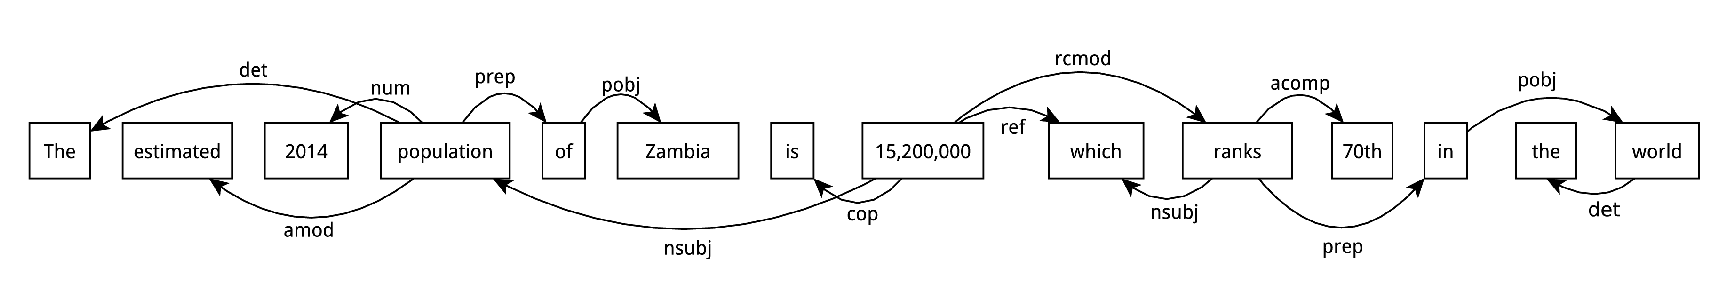
\includegraphics[width=0.7\textwidth]{images/dep.eps}
\end{figure}

\end{frame}

%------------------------------------------------

\begin{frame}
\frametitle{NumberRule}
\framesubtitle{Motivation}

\begin{block}{From \cite{shortestpathdep}}
If \textbf{$e_1$ and $e_2$ }are two entities mentioned in the same
 sentence such that they are observed to be in a \textbf{relationship R}, our hypothesis stipulates that the contribution of the sentence \textbf{dependency graph} to establishing the relationship $R(e_1, e_2)$ is almost \textbf{exclusively concentrated in the shortest path} between $e_1$ and $e_2$ in the undirected version of the dependency graph.
\end{block}
\begin{itemize}
\item When looking for clues for relation extraction, dependency path is a good place to start.
\item In the case of Numerical Relations, we already know what to look for: \textit{keywords}.
\item Need to take care of modifications to the entities, delta words
\end{itemize}
\end{frame}

%------------------------------------------------

\begin{frame}
\frametitle{NumberRule}
\framesubtitle{Definitions}
\begin{itemize}
\setlength\itemsep{\ntronitemsep}
 \item \textbf{Keywords}  Words that might help in identifying relations.(\textit{GDP}, \textit{internet}, \textit{inflation})
 \item \textbf{Delta words} Words that indicate that the mention expresses a change, and not the actual relation. \\ (\textit{change}, \textit{up}, \textit{down}, \textit{increased}, \textit{changed}, \textit{risen})
  \item \textbf{Modifiers} A word $m$ is said to be a modifier of the word $w$ if there is a modifying dependency from $m$ to $w$.\\ (\textit{blue} modifies \textit{whale} in \emph{\textbf{blue} whale}, \emph{\textbf{urban} population}).
%   \item \textbf{Augmented Phrase} For a word $W$, the \emph{Augmented Phrase} $W'$ is formed by concatenating $W$ with words $P$ such that $W$ and $P$ are related via a \emph{modifying dependency}. \\(for the word \textit{whale}, \textbf{\textit{blue whale}} is the augmented phrase)
\end{itemize}

\end{frame}

%------------------------------------------------
\begin{frame}[shrink=20]
\frametitle{NumberRule}
\framesubtitle{Extraction Algorithm}
	\begin{algorithmic}[1]

	\For{$(e, n) \in (E_S \times N_S)$} //For all entity-number pairs
 \State $P \gets$ words in dependency path between $e$ and $n$
 \For{$r \in R$}
 \If{$P \cap K_r = \emptyset$}
 \State continue;\ //keyword is not present
 \EndIf

 \If{$P \cap \Delta \not = \emptyset$} 
 \State continue;\ //delta words are present
 \EndIf

 \If{$Unit(n) \not \in LegalUnits(r)$} 
 \State continue;\ //incompatible units?
 \EndIf

\If{ $k_{r} \in P \cap K_{r}$ is modified/scoped}
\State continue; \ //keyword is modified/scoped
\EndIf

\If {e is modified/scoped}
\State continue; \ //entity is modified/scoped
\EndIf
 \State Extract $r(e, r, n)$.
 \EndFor
 \EndFor
 \end{algorithmic}
\end{frame}


%-------------------------------------------------------------
\begin{frame}
\frametitle{NumberRule}
\framesubtitle{NumberRule: Extractions}
%\subsection{Example}
\begin{itemize}
  \setlength\itemsep{1em}
\item ``The estimated population for 2014 of the {\color{blue}Australian} continent is about {\color{blue}36.25 million} people''

\item \tikzmark{}{{\color{blue}Australian}$\xrightarrow{amod}$continent$\xrightarrow{prep\_of}$2014
$\xrightarrow{prep\_for}$\emph{\color{green}\textbf{population}}$\xrightarrow{nsubj}$people$
\xrightarrow{num}$million$\xrightarrow{number}${\color{blue}36.25}}

\item ``The estimated population for 2014 of the {\color{blue}Australian} continent increased by about {\color{blue}3.25 million} people''

\item {\color{blue}Australian}$\xrightarrow{amod}$continent$\xrightarrow{prep\_of}$2014 $\xrightarrow{prep\_for}$\emph{\color{green}\textbf{population}}$\xrightarrow{nsubj}$ \textbf{\color{red}increased}$\xrightarrow{prep\_by}$people$\xrightarrow{num}$million $\xrightarrow{number}${\color{blue}36.25}
\end{itemize}
\end{frame}


\begin{frame}
\begin{table}
\begin{tabularx}{\textwidth}{b|s}
\hline
{\bf Sentence} & {\bf Test} \\
\hline
{\em The estimated population of Australia is about 36.25 million people. } & - \\
\hline
{\em The estimated population density of Australia is 36.25 million people {\bf per sq km.}} & Incompatible Units \\
\hline
{\em The estimated population of Australia {\bf increased} by about 36.25 million people. } & Delta Word Present \\
\hline
{\em The estimated population of {\bf urban} Australia is about 36.25 million people. } & Entity is Modified \\
\hline
{\em The estimated {\bf adolescent} population of  Australia is about 36.25 million. } & Keyword is Modified \\
\hline
\end{tabularx}
\caption{\label{fig:nr-eg} NumberRule outputs (Australia, Total Population, 36.25 million) only in the first sentence. The second column is test number that fails for other sentences. The input keyword is ``population''.}
\end{table}
\end{frame}
%------------------------------------------------

\section{NumberTron: Probabilistic Relation Extraction}
\part{NumberTron: Probabilistic Relation Extraction}
%Introduce graphical models here, tricky!
\newcommand{\vz}{{\mathbf z}}
\newcommand{\vn}{{\mathbf n}}
\newcommand{\cR}{{\cal R}}

\begin{frame}
\frametitle{NumberTron}
\begin{itemize}
 \item An Unlabeled Corpus (Sentencified, pruned to retain sentences having a country and a number)
 \item A Database of numerical facts, derived from data.worldbank.org.
 \item A Database of keywords
\end{itemize}
\begin{columns}[T] % align columns
\begin{column}{.48\textwidth}
\begin{adjustbox}{max width=\textwidth}
\begin{tabular}{|l|l|l|}
\hline
 Code & Num & Rel \\
\hline
/m/0hzlz&4.091616e+17&ELEC\\
/m/01nyl&9.27261850301&INF\\
/m/05qx1&2434964.0&POP\\
/m/03rt9&3538082.0&POP\\
/m/05v8c&22860078000.0&CO2\\
/m/07fsv&31824701.2783&GDP\\
/m/04w4s&32870000000.0&AGL\\
/m/035qy&15.5100261552&INF\\
/m/0d05q4&12.6628528269&INF\\
/m/088q4&1562886291.51&LIFE\\
\hline
\end{tabular}
\end{adjustbox}
\end{column}%
\hfill%
\begin{column}{.48\textwidth}
\begin{table}
\begin{adjustbox}{max width=\textwidth}
\begin{tabular}{|l|l|}
\hline 
 Relation & Keywords\\
\hline
 Internet User \% &internet\\
Land Area &area, land\\
Population &population, people, inhabitants\\
GDP & gross, domestic, GDP\\
$CO_2$ emission & carbon, emission, CO2, kilotons\\
Inflation & inflation\\
FDI &foreign, direct, investment, FDI\\
Goods Export & goods, export\\
Life Expectancy & life, expectancy\\
Electricity Production & electricity\\
\hline
\end{tabular}
\end{adjustbox}
\label{table:keywords}
\end{table}
\end{column}%

\end{columns}

\end{frame}

%------------------------------------------------
\begin{frame}
\frametitle{NumberTron}
\framesubtitle{Definitions}
For an entity $e$ (India)
\begin{itemize}
\setlength \itemsep{1em}
 \item One Graph \textbf{per entity}
 \item Let $S_e$ be the set of sentences that express the entity $e$.
 \item Let $Q_e$ denote the distinct numbers with unit that appear in $S_e$ \footnote{We use the unit tagger by \cite{sarawagi2014} to identity units of numbers in the text and to convert all
unit variants like "mile", "km" to a canonical SI unit, "meter".}
\item $\forall q \in Q_e$, let $S_{e,q} \subseteq S_e$ denote the sentences that mention $e$ and $q$. 
\end{itemize}
\end{frame}

%------------------------------------------------
\begin{frame}
\frametitle{NumberTron}
\framesubtitle{Definitions}
For  $e =$ (China)
\begin{itemize}
\setlength \itemsep{1em}
 \item $S_{china} = $  
 \{\textit{\color{blue}(i).. China says that annual inflation...to 4.3 percent, (ii)...China would initiate ... that its inflation rate ... 4.3 percent in October, (iii)...the number of chinese internet users has grown to 840 million...}\}
 \item $Q_{china} = $ \{4.3 percent, 840000000\}
\item $S_{china, 4.3 percent} = \{(i), (ii)\}$ 
\item $S_{china, 840000000} = \{(iii)\}$ 
\end{itemize}
\end{frame}


%------------------------------------------------
\begin{frame}
\frametitle{NumberTron}
\framesubtitle{Random Variables}
For each entity $e$, for each number $n_q$
\begin{itemize}
\item \textbf{$n_r^q$, number nodes} Binary, 1 if the number $q$ is related to $e$ via relation $r$. 
\end{itemize}
\vspace{3em}
For each mention, $s \in S_{e,q}$
\begin{itemize}
\item \textbf{$z_s$, mention nodes} multi-ary, can take values $r \in \cR = (R\, \cup \perp)$, set to $r \in R$ if the sentence expresses any of the $R$ relations, else set to $z_s = \perp$.
\end{itemize}
\end{frame}

%------------------------------------------------
\begin{frame}
\begin{columns}[T] % align columns
\begin{column}{.30\textwidth}
For  $e =$ (China)
\begin{itemize}
\setlength \itemsep{1em}
\item $S_{china} = \{(i), (ii), (iii)\}$  
\item $Q_{china} = $ \{4.3 \%, 840000000\}
\item $S_{china, 4.3 \%} = \{(i), (ii)\}$ 
\item $S_{china, 840000000} = \{(iii)\}$ 
\end{itemize}
\end{column}%

\hfill%

\begin{column}{.68\textwidth}
\begin{figure}
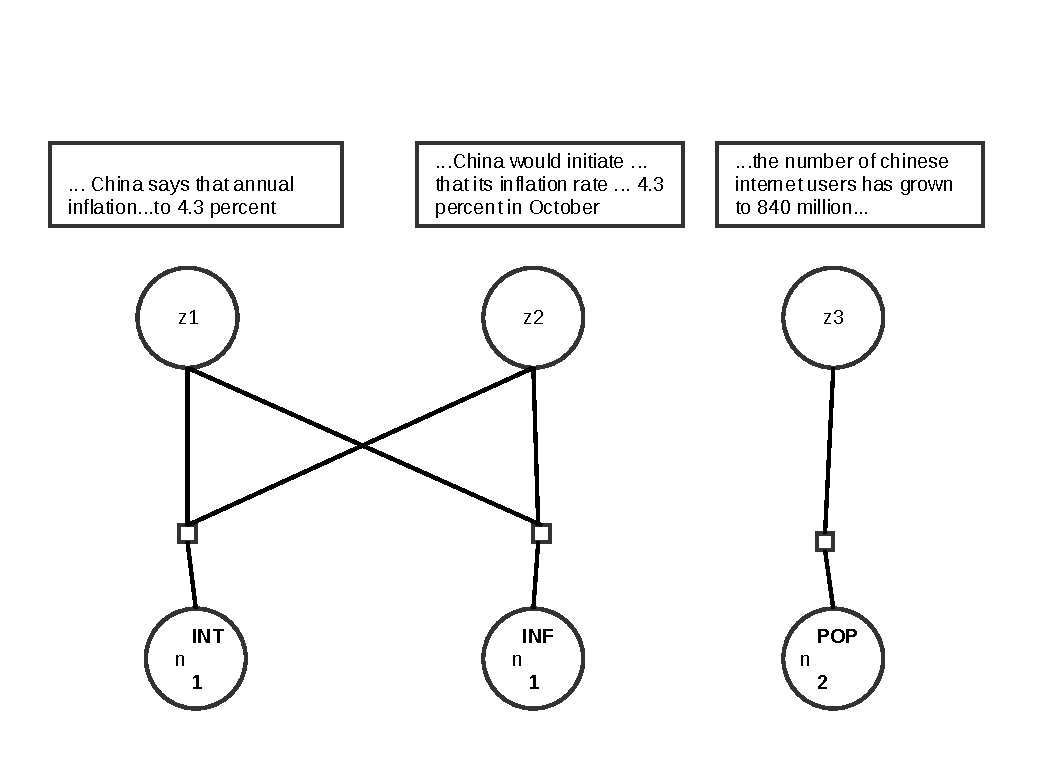
\includegraphics[width=0.7\textwidth]{images/numbertronmodel.eps}
\end{figure}
\end{column}%
\end{columns}
\end{frame}


%---------------------------------------------------
\begin{frame}
 \frametitle{NumberTron}
\framesubtitle{Graphical Model}
\begin{figure}
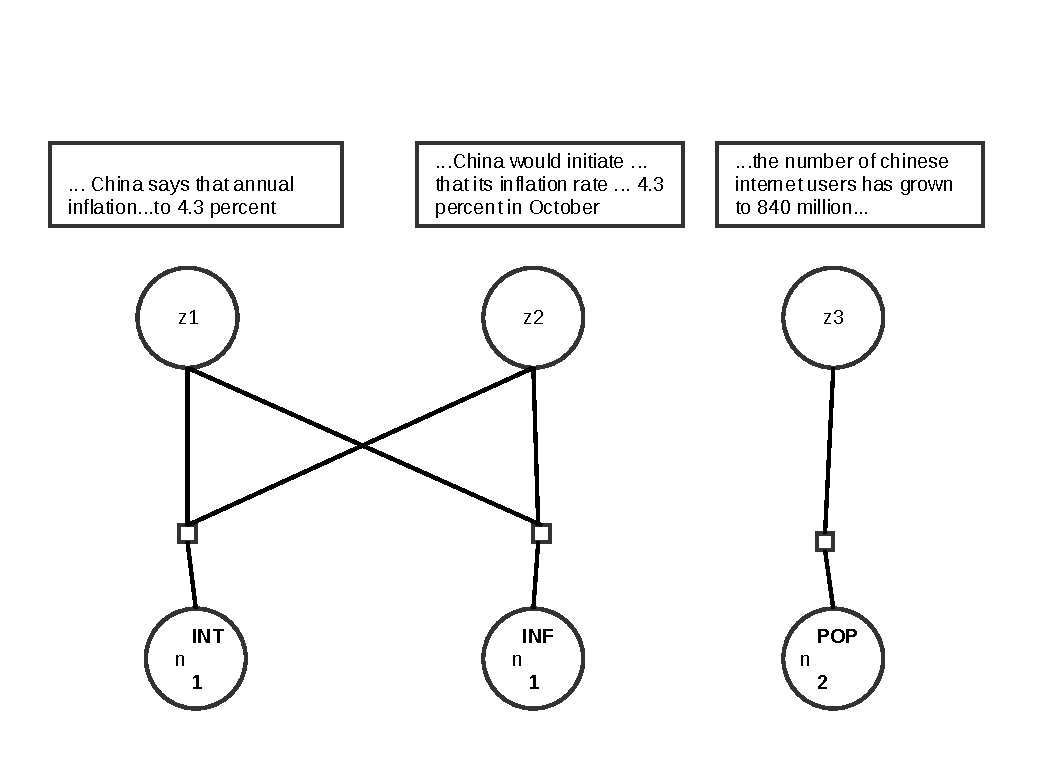
\includegraphics[width=0.7\textwidth]{images/numbertronmodel.eps}
\end{figure}

\end{frame}



%------------------------------------------------
\begin{frame}
\frametitle{NumberTron}
\framesubtitle{Features}
\begin{itemize}
\setlength \itemsep{2em}
\item \textbf{Mintz Features} Lexical and Synctactic features derived from POS tags and dependency path \cite{mintz}
\item \textbf{Keyword Features}
Derived from a pre-specified list of keywords per relation.
\item \textbf{Number Features} Capture Information on the magnitude, type (whole, fraction) can also be useful for relation extraction.
\end{itemize}

{\color{red}\emph{Afghanistan , which is mostly rural , has one of the lowest life expectancy rate in the world at 44 year for both man and woman}}. 

\end{frame}

%------------------------------------------------
\begin{frame}
\frametitle{NumberTron}
\framesubtitle{Features}
\begin{table}
\begin{tabular}{|l|l|}
\hline
Feature type & Features \\
\hline
Fixed Keywords & key: life	key: expect \\
\hline
Number Features & Num: Billion	Num: Integer \\
\hline
\end{tabular} \end{table}
  
{\color{red}\emph{Afghanistan , which is mostly rural , has one of the lowest life expectancy rate in the world at 44 year for both man and woman}}. 
\textit{The time ``44 year'' is converted to the SI unit, which comes out to be around 1.3 billion and thus the feature Num: Billion is fired.}

\end{frame}

\begin{frame}
\frametitle{NumberTron}
\framesubtitle{Features}
\begin{itemize}
\setlength \itemsep{1em}
\item \textit{inverse\_false$\vert$LOCATION$\vert$*LONG*$\vert$DURATION}, There is a long dependency path between the two entities, one of which is a location and other duration 
\item \textit{inverse\_false$\vert$B\_-2 B\_-1$\vert$LOCATION$\vert$*LONG*$\vert$DURATION$\vert$year for}, Same as above, but now with windows of text around entities of interest 
\item str:rural[rcmod]$->\vert$LOCATION$\vert$[nsubj]$->$have[root]$<-$at[prep]$<-$year[pobj]$<-\vert$DURATION , The typed dependency path 
\item dir:$->\vert$LOCATION$\vert-><-<-<-\vert$DURATION , Direction of dependencies 
\end{itemize}

{\color{red}\emph{Afghanistan , which is mostly rural , has one of the lowest life expectancy rate in the world at 44 year for both man and woman}}. 

\end{frame}


%------------------------------------------------
\begin{frame}
\frametitle{NumberTron Training}
\framesubtitle{Perceptron}
\begin{itemize}
\item The classical perceptron forms the core of our training procedure.
\end{itemize}
\begin{equation}
\theta \gets \theta + \eta * (t_i - o_i) * x_i
\end{equation}

\begin{gather}
   \mathterm[t1]{\theta}
   \gets
   \mathterm[t2]{\theta}   +
   \eta * (
   \mathterm[t3]{t_i} - 
   \mathterm[t4]{o_i} ) * 
   \mathterm[t5]{x_i} 
\end{gather}


\begin{itemize}
   \item  Weights \indicate[red]{t2}[out=0,in=-75]
   \item  True Label \indicate[blue]{t3}[out=0,in=-90]
   \item  Observed Label \indicate[yellow]{t4}[out=0,in=-90]
   \item  Feature (Binary) \indicate[green]{t5}[out=0,in=-90]
\end{itemize}
\end{frame}
%------------------------------------------------

%------------------------------------------------
\begin{frame}
\frametitle{NumberTron Training}
\framesubtitle{True Labels: Distant Supervision}
\begin{figure}
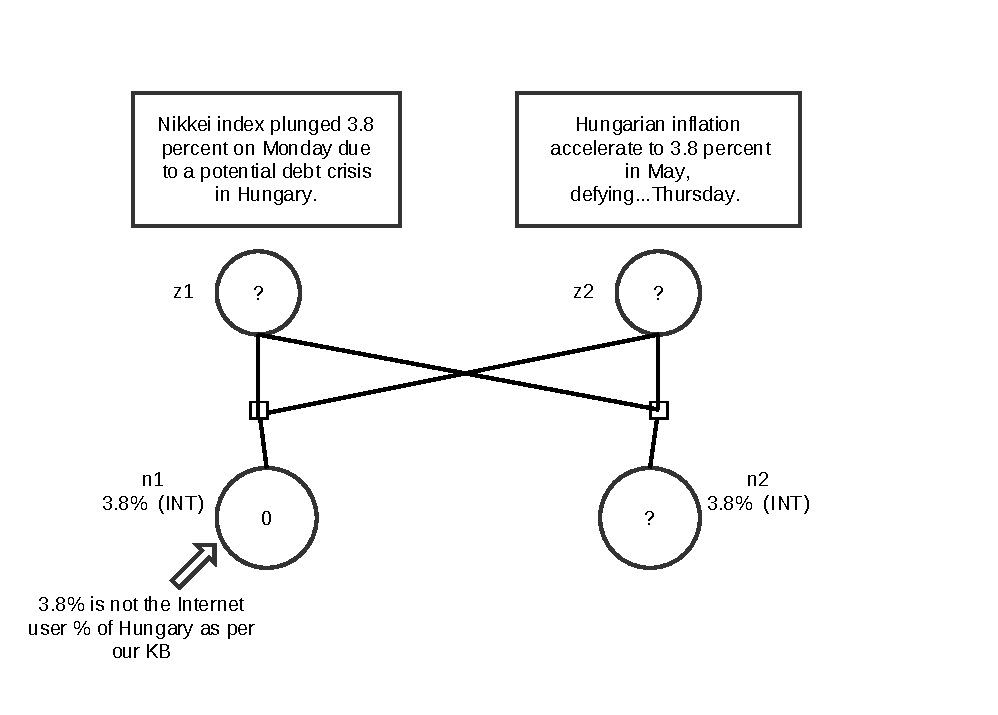
\includegraphics[width=\textwidth, height=0.8\textheight]{images/truelabel11.eps}
\end{figure}
\end{frame}
%------------------------------------------------

%------------------------------------------------
\begin{frame}
\frametitle{NumberTron Training}
\framesubtitle{True Labels: Distant Supervision}
\begin{figure}
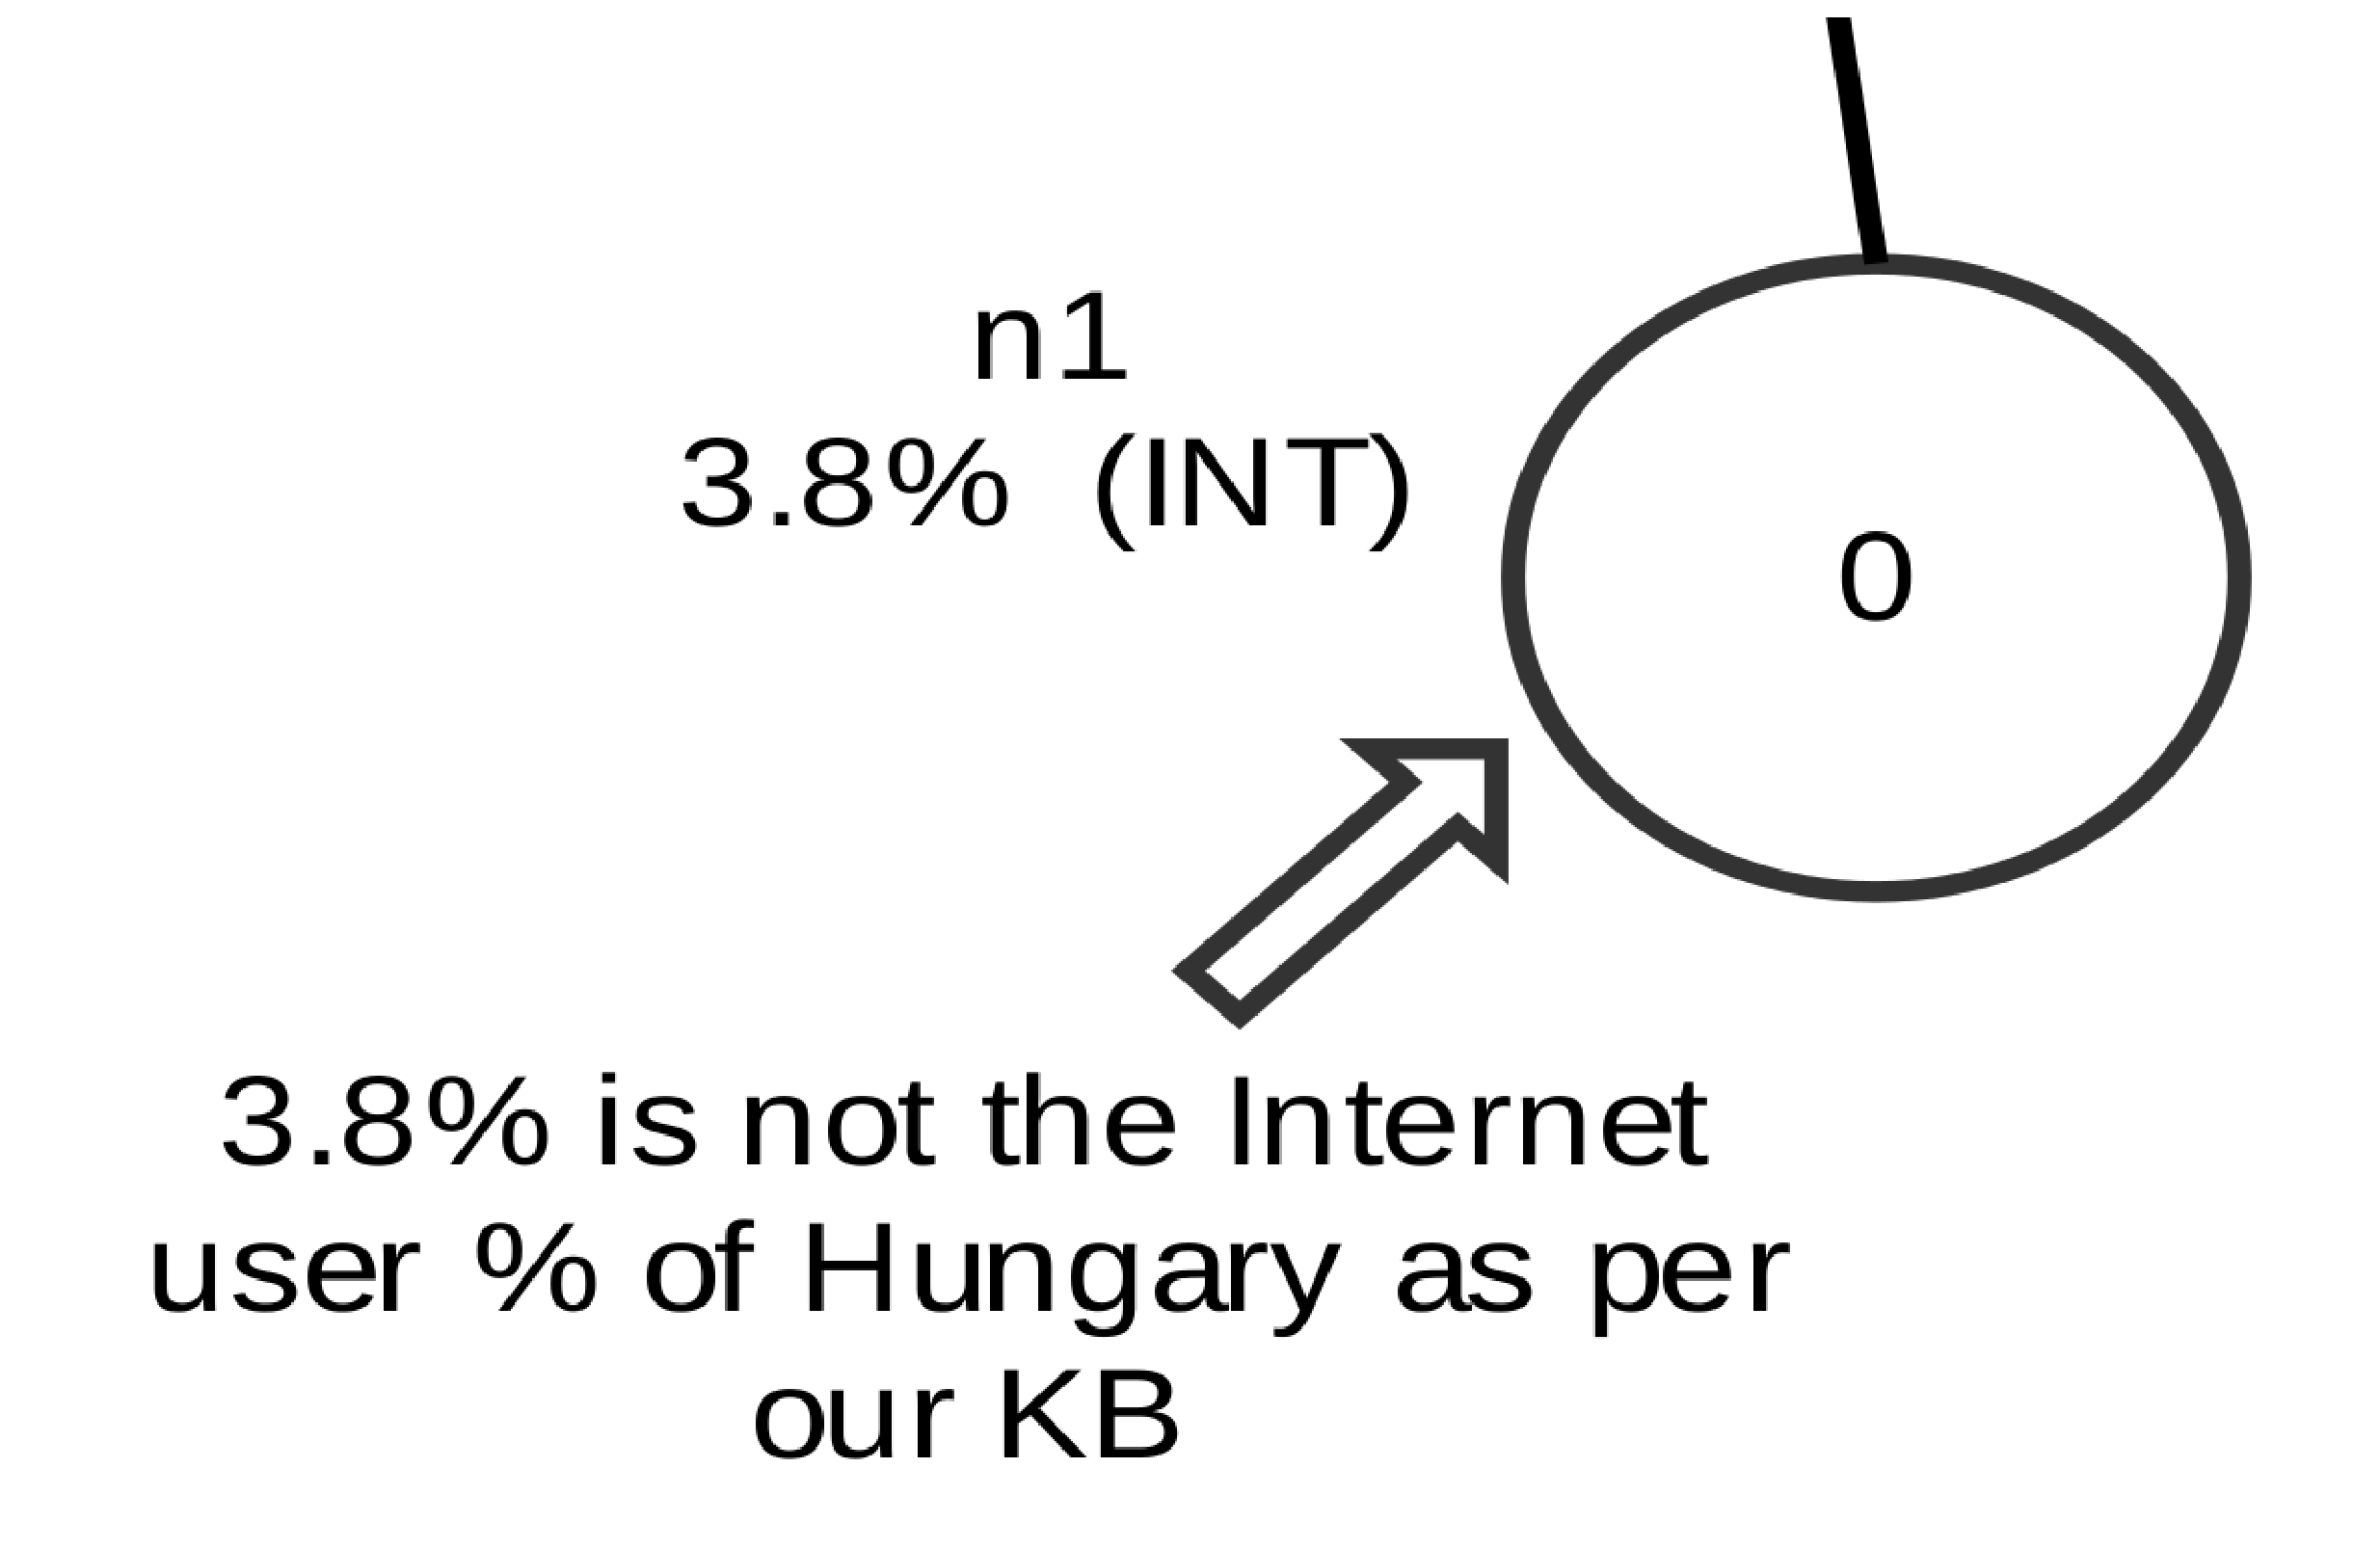
\includegraphics[width=0.4\textwidth, height=0.4\textheight]{images/matching.eps}
\end{figure}
\begin{itemize}
 \item Is 3.8\% within $\delta\%$ of the values in the knowledge base for Internet User Percent of Hungary?
 \item $\delta = 20$
\end{itemize}

\end{frame}
%------------------------------------------------

%------------------------------------------------
\begin{frame}
\frametitle{NumberTron Training}
\framesubtitle{True Labels: Distant Supervision}
\begin{figure}
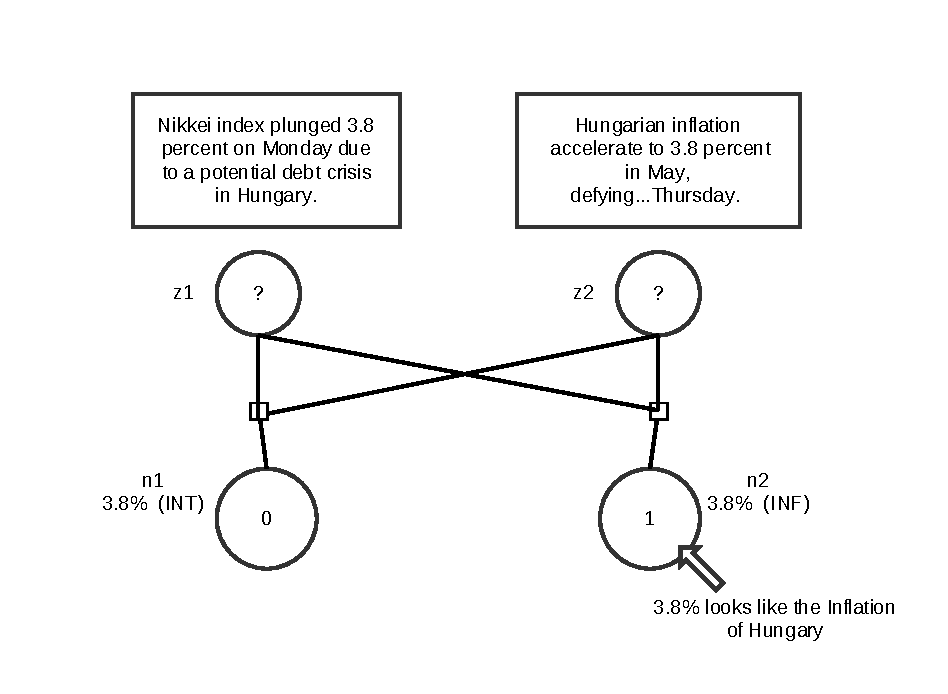
\includegraphics[width=\textwidth, height=0.8\textheight]{images/truelabel12.eps}
\end{figure}
\end{frame}
%------------------------------------------------


%------------------------------------------------
\begin{frame}
\frametitle{NumberTron Training}
\framesubtitle{True Labels: Distant Supervision}
\begin{figure}
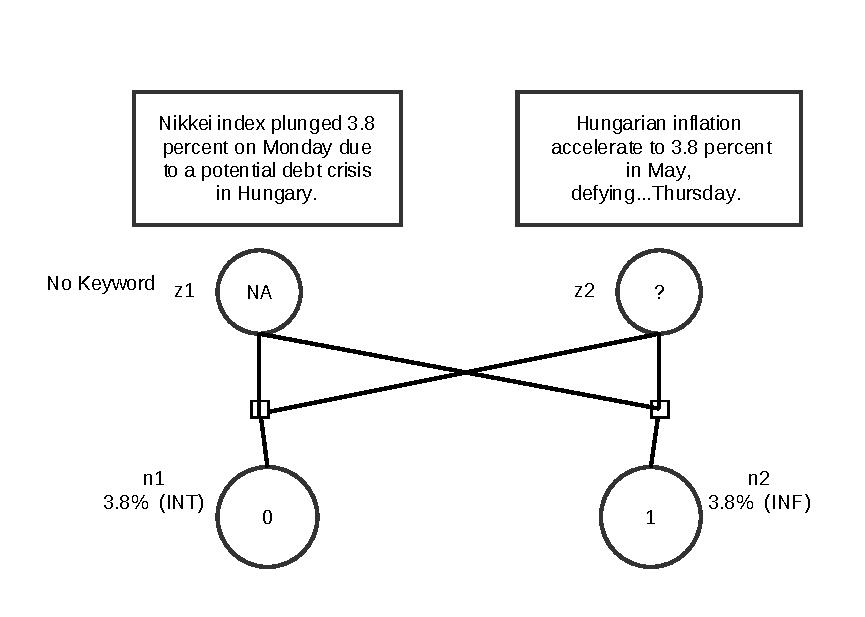
\includegraphics[width=\textwidth, height=0.8\textheight]{images/truelabel13.eps}
\end{figure}
\end{frame}
%------------------------------------------------


%------------------------------------------------
\begin{frame}
\frametitle{NumberTron Training}
\framesubtitle{True Labels: Distant Supervision}
\begin{figure}
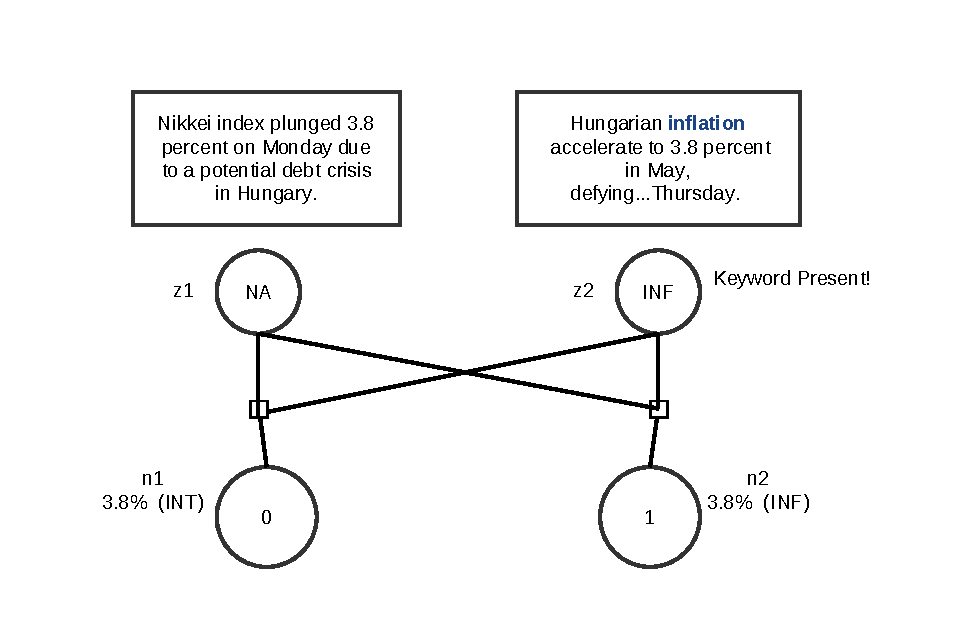
\includegraphics[width=\textwidth, height=0.8\textheight]{images/truelabel14.eps}
\end{figure}
\end{frame}
%------------------------------------------------


%------------------------------------------------
\begin{frame}
\frametitle{NumberTron Training}
\framesubtitle{Observed Labels: Full Inference}
\begin{figure}
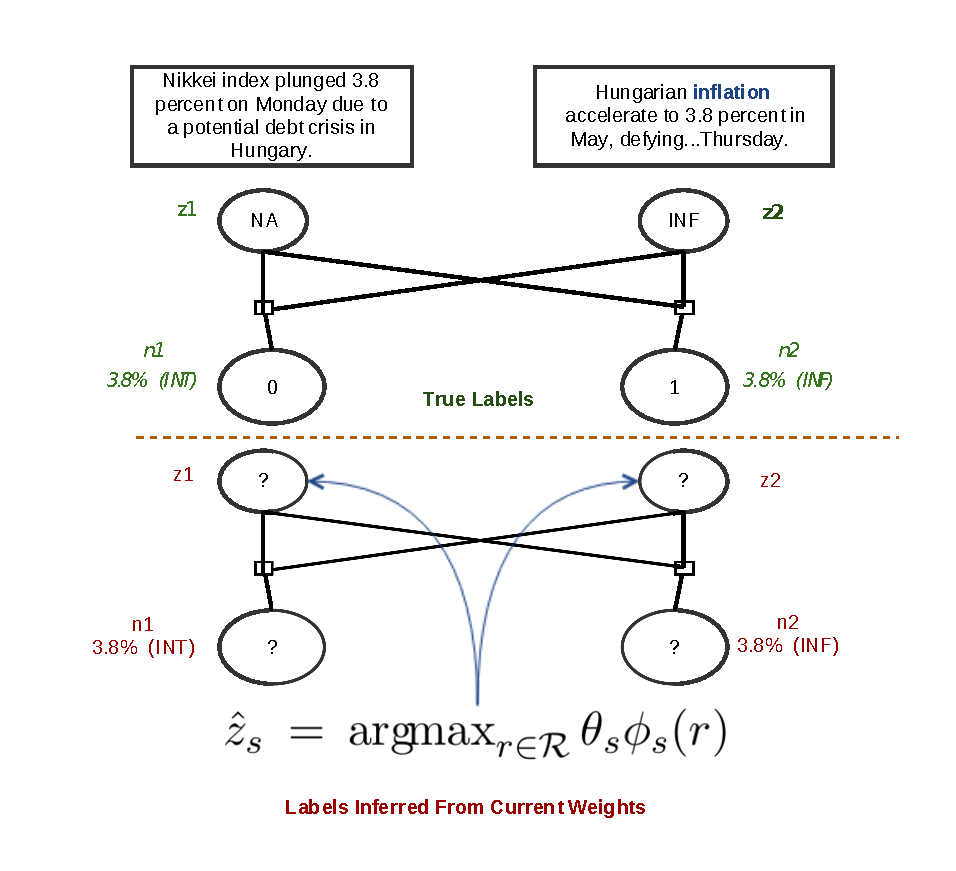
\includegraphics[width=\textwidth, height=0.85\textheight]{images/fullinf_1.eps}
\end{figure}
\end{frame}
%------------------------------------------------


%------------------------------------------------
\begin{frame}
\frametitle{NumberTron Training}
\framesubtitle{Observed Labels: Full Inference}
\begin{figure}
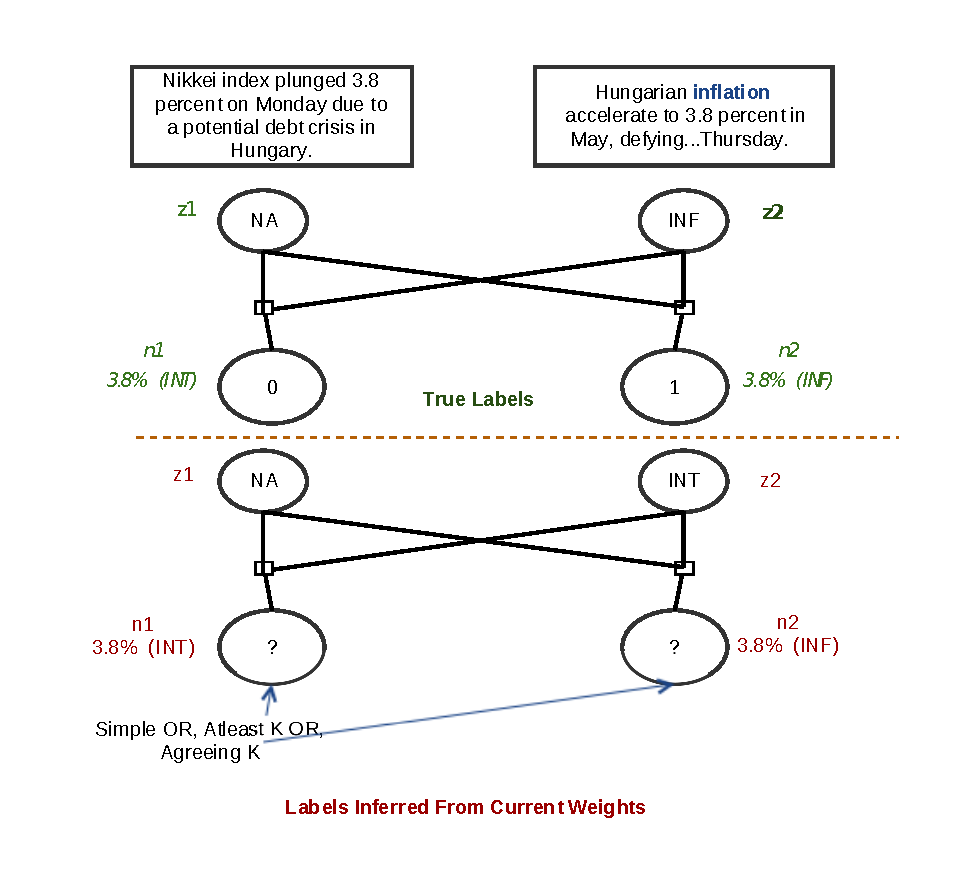
\includegraphics[width=\textwidth, height=0.85\textheight]{images/fullinf_2.eps}
\end{figure}
\end{frame}
%------------------------------------------------


%------------------------------------------------
\begin{frame}
\frametitle{NumberTron Training}
\framesubtitle{Observed Labels: Full Inference}
\begin{figure}
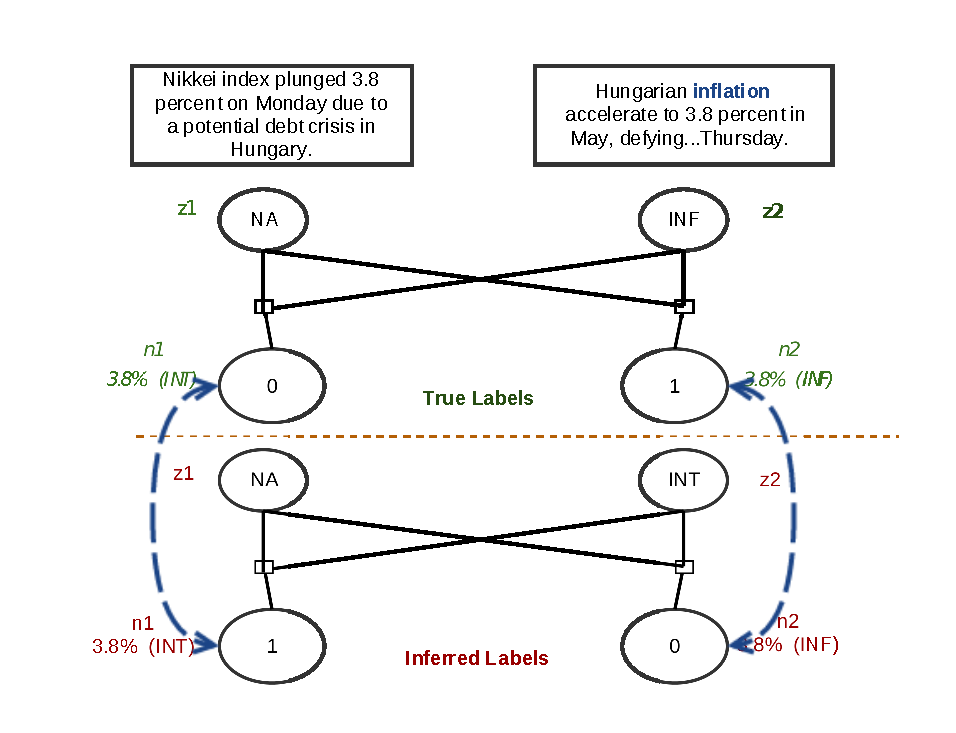
\includegraphics[width=\textwidth, height=0.85\textheight]{images/fullinf_3.eps}
\end{figure}
\end{frame}
%------------------------------------------------


%------------------------------------------------
\begin{frame}
\frametitle{NumberTron Training}
\framesubtitle{Observed Labels: Full Inference}
\begin{figure}
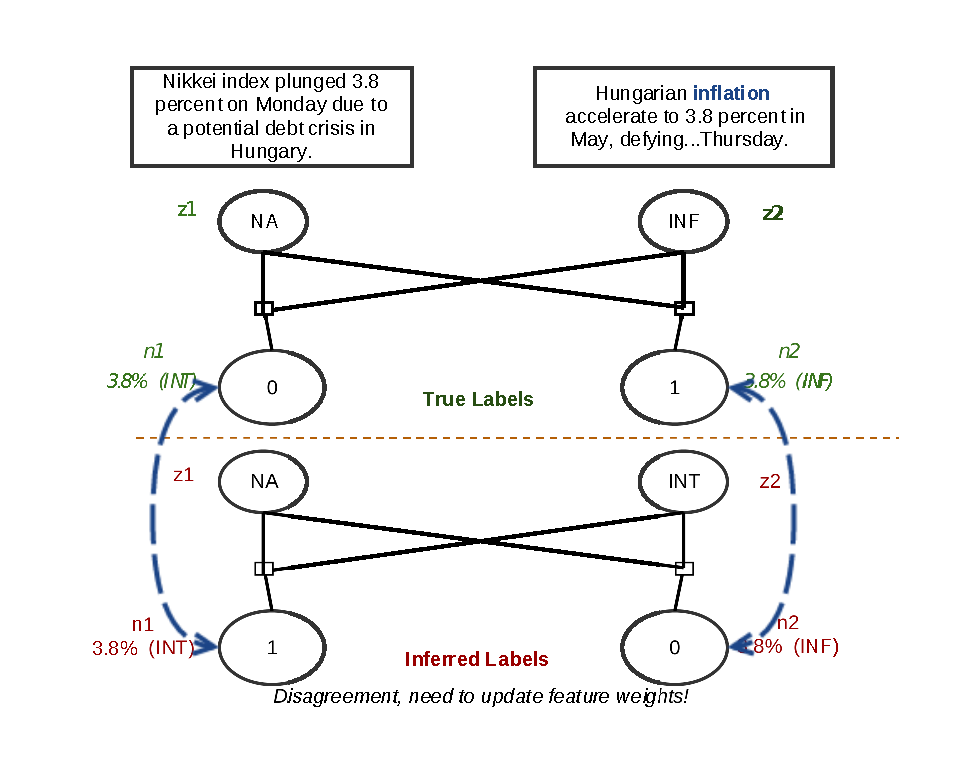
\includegraphics[width=\textwidth, height=0.85\textheight]{images/fullinf_4.eps}
\end{figure}
\end{frame}
%------------------------------------------------


%------------------------------------------------
\begin{frame}
\frametitle{NumberTron Training}
\framesubtitle{Updating Feature Weights}
\begin{itemize}
\setlength{\itemsep}{1em}
\item Let $f_1, f_2, ..., f_k$ be the features fired for \textit{Hungarian inflation  accelerate to 3.8 percent in May, defying...Thursday.}
\item Examples: \textbf{key: inflation}, \textbf{Num: Units} and so on.
\item $\theta_{f_i}^{INT} \gets \theta_{f_i}^{INT} - 1$
\item $\theta_{f_i}^{INF} \gets \theta_{f_i}^{INF} + 1$
\item These features actually indicate inflation relation, and not the internet relation!
\end{itemize}
\end{frame}
%------------------------------------------------


%------------------------------------------------
\begin{frame}
\frametitle{NumberTron}
\framesubtitle{Extraction}
\begin{itemize}
 \item \textbf{Sentence Level Extractions}
 
\item Given a sentence S, let $E$ be the set of entities and $Q$ be the set of numbers that are present in the sentence.  
\item We then calculate a score$(r,e,q)$ for a $e \in E$ and $q \in Q$ for being tagged $r$ as $\theta^r_q \phi_q(n_q=1) + \theta_s \phi_s(r)$
where $\phi_s$ captures the features in sentence $S$ tied to entity $e$ and number $q$.
\item For each $(e,q)$ we assign a label $r$ if the min-max normalized score is greater than some threshold $\alpha$.
\item We use a cross validation set to obtain the $\alpha$ = 0.90.
\end{itemize}

\end{frame}

%------------------------------------------------

\section{Results}
\begin{frame}
\frametitle{Experiments}
\framesubtitle{Training Corpus}

\begin{itemize}
\item Tac KBP 2014 corpus comprising roughly 3 million documents from NewsWire, discussion forums, and the Web.
\item Knowledge base is compiled from data.worldbank.org
\begin{itemize}
\item Dataset contains 1,281 numeric indicators for 249 countries, with over 4 million base facts.
\item Dataset is normalized by converting all the values to their SI base unit value.
\end{itemize}
\end{itemize}

\end{frame}

%--------------------------------------------------

\begin{frame}
\frametitle{Experiments}
\framesubtitle{Test Set}

\begin{itemize}
\item Mix of 430 sentences from TAC corpus and sentences from Web search on relation name.
\end{itemize}

\begin{small}
\begin{table}[h]
\centering
%     \begin{adjustbox}{width=\textwidth,center}
    % \begin{adjustbox}{center}
     \begin{adjustbox}{max width=\textwidth}
        \begin{tabular}{|l|c|c|c|}
            \hline
             \textbf{Relation} &  \textbf{Units} & \textbf{Positive} &  \textbf{Negative} \\
            \hline
            \hline
             Land Area & Sq. Km & 57 &  17 \\
            \hline
             Population & - & 51 &  300 \\
            \hline
            
            \multicolumn{1}{|l|}{Inflation}  & \multicolumn{1}{c}{percent} & \multicolumn{1}{|c|}{51} & \multirow{2}{*}{84} \\\cline{1-2}
            \multicolumn{1}{|l|}{Internet Users} & \multicolumn{1}{c}{percent} & \multicolumn{1}{|c|}{15} & \\\cline{1-2} 
            
            \hline
            
            \multicolumn{1}{|l|}{FDI} & \multicolumn{1}{c}{\$ (USD)} & \multicolumn{1}{|c|}{10} & \multirow{3}{*}{35} \\\cline{1-2}
            \multicolumn{1}{|l|}{GDP} & \multicolumn{1}{c}{\$ (USD)} & \multicolumn{1}{|c|}{8} & \\\cline{1-2}
            \multicolumn{1}{|l|}{Goods Export} & \multicolumn{1}{c}{\$ (USD)} & \multicolumn{1}{|c|}{11} & \\\cline{1-2}
            
            \hline
             Life Expectancy & year & 15 &  34 \\
            \hline
             Electricity Production & kWh & 13 &  6 \\
            \hline
             $CO_{2}$ Emissions & kiloton &  8 &  16\\
            \hline
        \end{tabular}
	\end{adjustbox}
%     \vspace{ - 05 mm}
    \caption{Test corpus statistics: The third column is the number of instances per relation and the fourth column is the number of "none-on-the-above" ($\perp$) grouped by relation of the same unit.}
    \label{tab:test_data_stats}
\end{table}
\end{small}

\end{frame}


%----------------------------------------------------

\begin{frame}
\frametitle{Baseline Algorithms}
\begin{itemize}
\setlength\itemsep{2em}
\item \textbf{Recall \textendash Prior Baseline: } For each unit, predict the relation with the highest \emph{test} prior ignoring the "none-of-the-above" class.
\begin{small}
\begin{table}[h]
\centering
%     \begin{adjustbox}{width=\textwidth,center}
    % \begin{adjustbox}{center}
     \begin{adjustbox}{max width=\textwidth}
        \begin{tabular}{|l|c|c|c|}
            \hline
            
            \multicolumn{1}{|l|}{Inflation}  & \multicolumn{1}{c}{percent} & \multicolumn{1}{|c|}{51} & \multirow{2}{*}{84} \\\cline{1-2}
            \multicolumn{1}{|l|}{Internet Users} & \multicolumn{1}{c}{percent} & \multicolumn{1}{|c|}{15} & \\\cline{1-2} 
            
            \hline
        \end{tabular}
	\end{adjustbox}
%     \vspace{ - 05 mm}
   
\end{table}
\end{small}

\begin{itemize}
	\item All the numbers with the unit "percent" will be labeled 'Inflation' since it is most frequent class 
	ignoring the "none-of-the-above" class. \pause
\end{itemize}


\item \textbf{MultiR ++ : Adapting MultiR for Numerical Relations}
\begin{itemize}
\item Added unit tagger as in our algorithms for identifying and normalizing numbers and units.
\item Added our partial matching (using $\pm \delta_r\%$) technique in distant supervision.
\end{itemize}
\end{itemize}
\end{frame}

%---------------------------------------------------
\begin{frame}
\frametitle{Results}
\framesubtitle{Numbertron vs NumberRule vs Baselines}

\begin{figure}
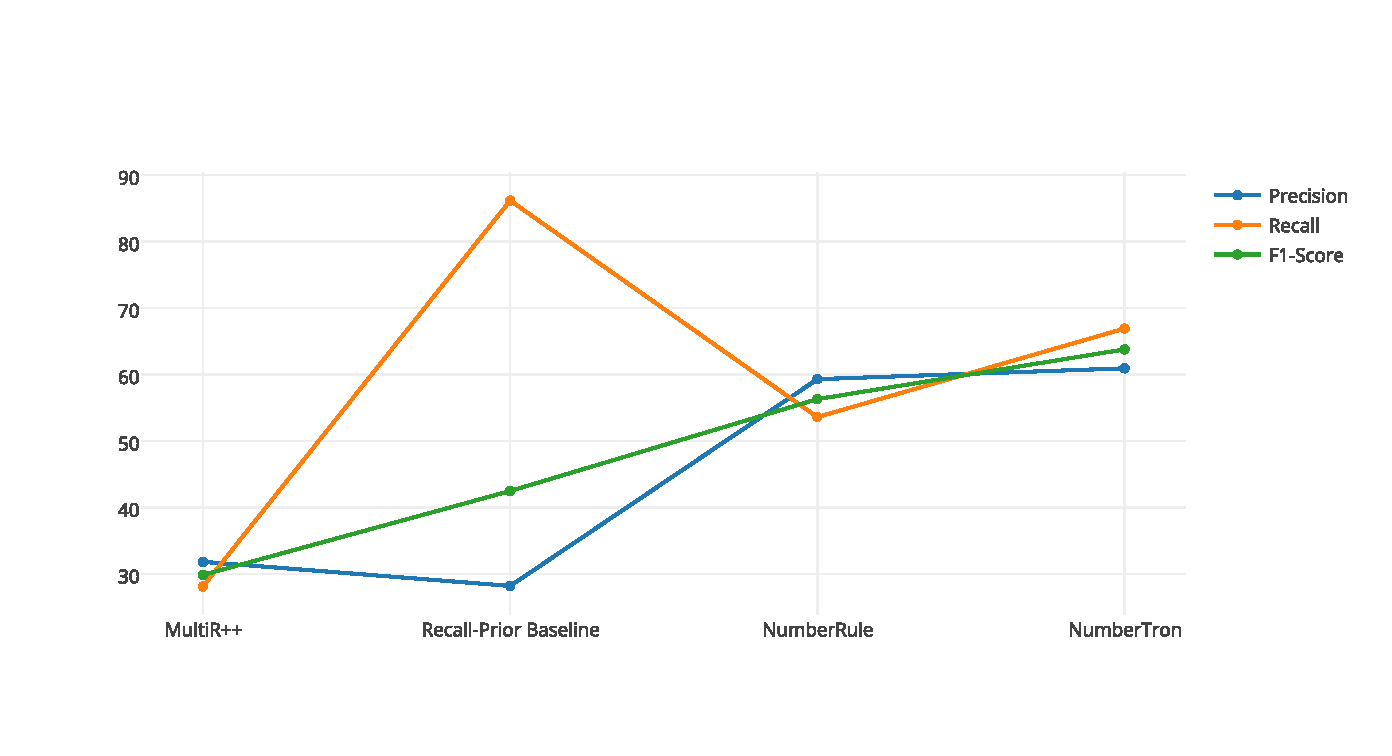
\includegraphics[width=0.7\textwidth]{images/main_comparison.eps}
\end{figure}

\begin{itemize}
\item Statistical method like NumberTron outperforms NumberRule on increased recall, which jumps from 53.6\% to 67\%
\item MultiR++ performs poorly because it does not model peculiarities of numerical relations.
\end{itemize}
\end{frame}
%---------------------------------------------------
\begin{frame}
\frametitle{Analysis}
\framesubtitle{NumberTron vs NumberRule}

\begin{itemize}
	\item NumberRule's missed recall is primarily because of not having a keyword on the dependency path.
    \begin{itemize}
    \setlength\itemsep{1em}
    	\item "{\em Turkey's central bank said Wednesday it expects the annual inflation rate to reach 6.09 percent at the end of 2009 , lower than the official target of 7.5 percent.}"
        \item Turkey $\xrightarrow{poss}$ bank $\xrightarrow{nsubj}$ said $\xrightarrow{ccomp}$ expects $\xrightarrow{xcomp}$ reach $\xrightarrow{dobj}$ percent $\xrightarrow{num}$ 6.09
        \item Since keyword 'inflation' is not on the shortest dependency path between Turkey and 6.09, NumberRule does not extract.
        \item Since NumberTron combines evidences from multiple features such as number's range, presence of 'inflation' in context and dependency path features.
    \end{itemize}
\end{itemize}


\end{frame}
%---------------------------------------------------

\begin{frame}
\frametitle{Ablation tests}
\framesubtitle{of various configurations of NumberTron}

\begin{table}
\begin{adjustbox}{max width=\textwidth}
\begin{tabular}{|l|ccc|ccc|ccc|}
%\begin{small}
\hline
%\textbf{Keyword Features} & 
\textbf{Distant Supervision} &  \multicolumn{3}{|c|}{\textbf{Simple OR}} &  \multicolumn{3}{|c|}{\textbf{Atleast-K}} & \multicolumn{3}{|c|}{\textbf{Agreeing-K}} \\
\hline
	    & P & R & F1 & P & R & F1 & P & R & F1\\
\hline 
\hline

%Fixed Keywords &
KB & 43.24 & 50.93 & 46.54 & 40.05 & 53.93 & 45.97 & 35.20 & 44.52 &  39.35\\
\hline
%Fixed Keywords & 
Keywords & 43.35 & 73.22 & 54.46 & 43.69 & 73.62 & 54.83 & 45.97 & 70.80 & 55.74 \\
\hline
%Fixed Keywords & 
KB + Keywords & 61.56 & 64.96 & 63.21 & 60.93 & 66.92 & 63.78 & 63.46 & 60.21 & 61.79\\
\hline

\end{tabular}
\end{adjustbox}
\caption{Comparison of various configurations for NumberTron}
\label{table:numbertronconfigs}
%\end{small}
\end{table}

\begin{itemize}
\item Keywords are crucial and KB in conjunction with keyword-based labeling adds significant value.
\end{itemize}

\end{frame}

%---------------------------------------------------

\begin{frame}
\frametitle{Ablation tests}
\framesubtitle{of feature templates for NumberTron}

\begin{table}
\begin{tabular}{|l|c|c|c|}
%\begin{small}
\hline
Features & Precision & Recall & F1-score \\
\hline
\hline
Mintz features only & 22.85 & 36.86 & 28.21 \\
\hline
Keyword features only & 51.24 & 52.55 & 51.89 \\
\hline
Mintz + Keyword & 47.10 & 39.04 & 42.71\\
\hline
Mintz + Number & 17.80 & 35.03 & 23.67 \\
\hline
Keyword + Number & 45.15 & 69.70 & 54.80\\
\hline
Mintz + Keyword + Number & \emph{60.93} & \emph{66.92} & \emph{63.78}\\
\hline
\end{tabular}
\caption{Ablation tests of feature templates for NumberTron}
\label{tab:ablationtests}
%\end{small}
\end{table}

\begin{itemize}
\item Large set of Mintz features confuses the classifier; Keyword features are much effective in learning.
\end{itemize}


\end{frame}
%---------------------------------------------------
\begin{frame}
\frametitle{Results}
\framesubtitle{NumberTron vs NumberRule}

\begin{figure}
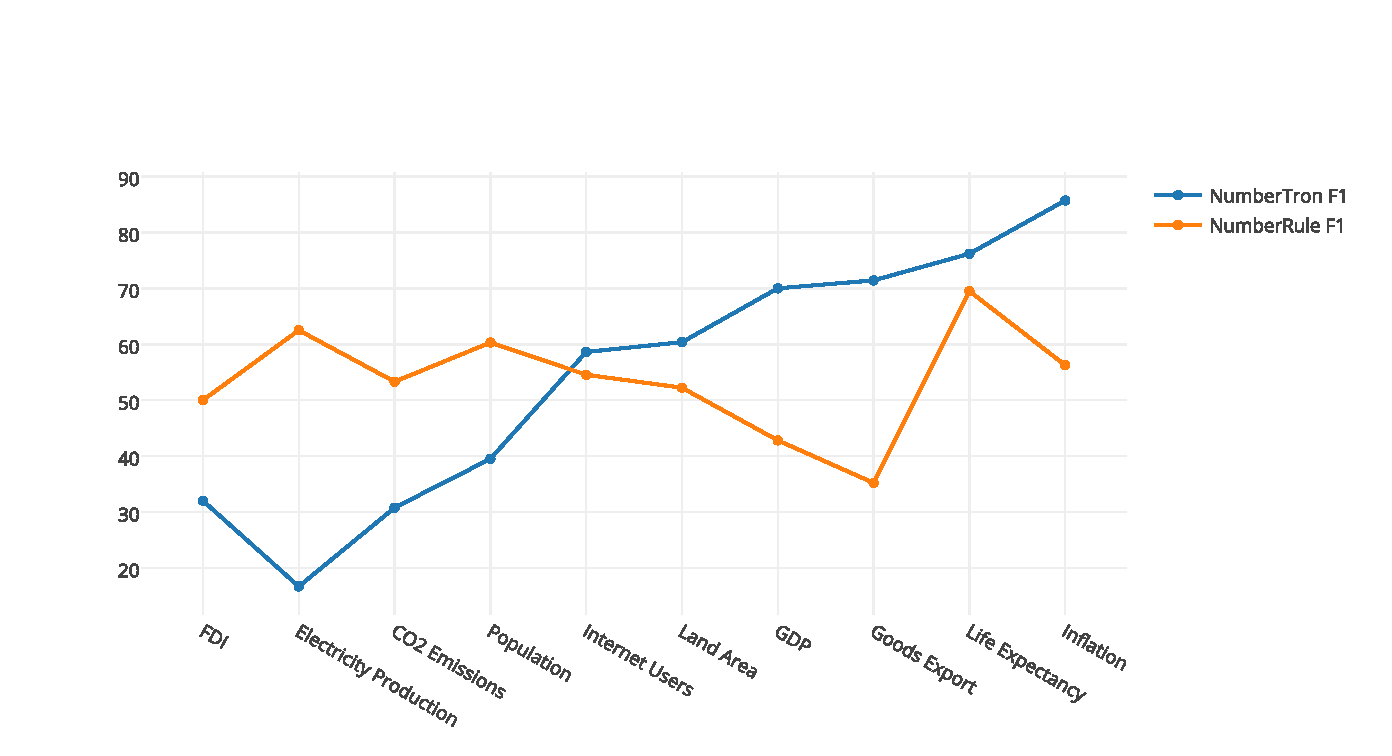
\includegraphics[width=0.7\textwidth]{images/per_relation.eps}
\caption{Per relation F1 scores for NumberRule and best configuration of NumberTron}
\label{tab:perrelscore}
\end{figure}

\end{frame}
%---------------------------------------------------
% \begin{frame}
% \frametitle{Analysis}
% \framesubtitle{per relation analysis of NumberTron vs NumberRule}
% \begin{itemize}
% \setlength\itemsep{1em}
% \item For relations like FDI, Electricity production, and $CO_2$ emissions, NumberTron performs poorly because of the lack of the training data in the corpus.
% \item Inflation and Population are well represented in training corpus and hence higher recall.
% 
% \end{itemize}
% \end{frame}
%---------------------------------------------------

%---------------------------------------------------
\section{Summary and Future Work}	
\begin{frame}
\frametitle{Future Work}
\begin{itemize} 
\setlength \itemsep{1em}
\item \textbf{Temporal Modeling} Many of the relations that we target are time dependent.
\item \textbf{Soft constraints in NumberTron} Instead of hardcoding true assignments to the random variables, we can think of an alternative scheme in which the keyword nodes are added to the graphical model along with edge potentials that capture the similarity between potential relation and the keywords.
\item \textbf{Extracting with Delta Words} NumberTron and NumberRule ignore mentions that express a change rather than the absolute fact.
\end{itemize}
\end{frame}

\begin{frame}
\frametitle{Summary}
\begin{itemize} 
\item  Numerical relation extraction has several peculiarities, more challenging than standard IE.
\item \textbf{NumberRule}, a rule based system that can extract any numerical relation given input keywords for that relation.
\item \textbf{NumberTron}, a probabilistic graphical model, that employs novel task-specific features and can be trained via distant supervision or other heuristic labelings. 
\item NumberTron aggregates evidence from multiple features and produces higher recall at a precision comparable to NumberRule. 
\item Both systems vastly outperform baselines and non-numeric IE systems, with NumberTron yielding over 33 point F-score improvement.
\end{itemize}
    
\end{frame}


\section{Thanks!}
%----------------------------------------------------------------------------------------
\begin{frame}[allowframebreaks]
        \frametitle{References}
        \bibliographystyle{amsalpha}
        \bibliography{numrel.bib}
\end{frame}

\begin{frame}
\frametitle{Summary}
\framesubtitle{NumberTron vs NumberRule}
\begin{tabularx}{\textwidth}{|b |b |b |}
\hline
  & \textbf{NumberRule} &  \textbf{NumberTron}\\ \hline
 \textbf{Idea} & Use dep path between the number and the entity in the mention& A Graphical Model with Perceptron like training algorithm\\ \hline
 \textbf{Supervision}& Relation specific keywords. & Relation specific keywords + Numerical knowledge base. \\ \hline
 \textbf{Handling False +ves}&  Look for relation specific keywords in the dep path.&  Keyword features. \\ \hline
\textbf{Handling Mentions Expressing Change}& No extraction if a delta word exists on the dep path. &  Remove sentences having delta words on the dep path\\ \hline 

 \end{tabularx}
\end{frame}

\begin{frame}
\frametitle{NumberTron vs NumberRule}
\begin{tabularx}{\textwidth}{|b |b |b |}
\hline
\textbf{Use of Unit Tagger} & Used to test compatibility of a relation and the number.& Used for training data creation and flattening to SI units.\\ \hline
 \textbf{Common Number Pruning} & N/A & Features included to capture type (whole, fraction), magnitude and frequency. \\ \hline
 \textbf{Modified Relations} & Handled by attaching words related via modifying dependencies, \emph{urban} population.& Not handled in the model, can be handled at the time of extraction using a similar scheme. \\ \hline
  \textbf{Results} & P = 59.30, R = 53.60, F-Score = 56.30& P = 60.93, R = 66.92, F-Score = 63.78\\ \hline
\end{tabularx}
\end{frame}

\end{document}